\documentclass[12pt]{report}
\usepackage[utf8]{inputenc}
\usepackage{blindtext}
\usepackage{lmodern}
\usepackage[T1]{fontenc}
\usepackage{graphicx}
\usepackage{ragged2e}
\usepackage[
	a4paper,
	left=20mm,
	top=20mm,
	]{geometry}
\usepackage[breaklinks]{hyperref}
\usepackage{amsthm}
\usepackage{microtype}
\usepackage{parskip}
\usepackage{enumitem,amssymb}
\usepackage{makecell}
\usepackage{amsmath}
\usepackage{stackengine}
\usepackage{enumitem}
\usepackage{xcolor}
\usepackage{mathtools}
\usepackage{pdfpages}
\usepackage{wrapfig}
\usepackage{subcaption}
\usepackage{setspace}
\usepackage{pgffor, ifthen}
\usepackage{multicol}
\usepackage{titlesec}
	\titleformat{\chapter}[hang] 
	{\normalfont\huge\bfseries}{\chaptertitlename\ \thechapter:}{1em}{} 
\graphicspath{ {assets/} }
\titlespacing{\chapter}{0pt}{-16pt}{1cm}%

% ==================
% Custom Functions
% ==================

% Usage: \notes[10pt]{3}{\textwidth}
\newcommand{\notes}[3][\empty]{%
    \noindent\vspace{-0.25cm}\\
    \foreach \n in {1,...,#2}{%
        \ifthenelse{\equal{#1}{\empty}}
            {\rule{#3}{0.5pt}\\}
            {\rule{#3}{0.5pt}\vspace{#1}\\}
        }
    \vspace{-1cm}
}

%% Options
\newboolean{@answer}
\DeclareOption{noanswers}{\setboolean{@answer}{false}}
\DeclareOption{answers}{\setboolean{@answer}{true}}
\ExecuteOptions{noanswers}
\ProcessOptions*

%% Real-time switching
\DeclareRobustCommand{\showanswers}{\setboolean{@answer}{true}}
\DeclareRobustCommand{\noshowanswers}{\setboolean{@answer}{false}}
\noshowanswers

\DeclareRobustCommand{\StudentVSpace}[1]{%
	\ifthenelse{\boolean{@answer}}{}{\vspace{#1}}
}

%% Fill in blanks
\DeclareRobustCommand{\fillinunderline}[1]{%
\ifthenelse{\boolean{@answer}}{\textcolor{red}{\underbar{~~~ #1 ~~~}}}{\textcolor{gray}{\underbar{\phantom{~~~ #1 ~~~}}}}%
}

\DeclareRobustCommand{\fillinspace}[1]{%
\ifthenelse{\boolean{@answer}}{\textcolor{red}{#1}}{\phantom{#1}}%
}

\DeclareRobustCommand{\fillinblank}[1]{%
\ifmmode\begingroup\@ifstar{\fillinunderline{#1}}{\fillinspace{#1}}\endgroup%
\else\begingroup\@ifstar{\fillinspace{#1}}{\fillinunderline{#1}}\endgroup%
\fi}

%% A large blank spaces or answers
%\DeclareRobustCommand{\answerspace}[2]{\ifthenelse{\boolean{@answer}}{#2}{\vspace{#1}}}
\newsavebox{\answerspacebox}
\newlength{\answerspaceheight}
\DeclareRobustCommand{\answerspace}[1]{%
	\newline
	\sbox{\answerspacebox}{\parbox{\columnwidth}{#1}}
	\setlength{\answerspaceheight}{\ht\answerspacebox}	% Height
	\addtolength{\answerspaceheight}{\dp\answerspacebox}% Depth
	\ifthenelse{\boolean{@answer}}{\usebox{\answerspacebox}}{\vspace{\answerspaceheight}}%
}

% Usage
%\begin{choices}[itemsep=10pt]
%	\item
%	\item
%	\item
%\end{choices}
\newlist{choices}{enumerate}{1}
\setlist[choices]{label*=(\Alph*)}
\newcommand{\choice}{\item}

\hypersetup{
	colorlinks=true,
	linkcolor=blue,
	filecolor=blue,
	urlcolor=blue,
}

% Usage
% \fillinunderline{atom}
\newcommand\fillin[1]{
	\sbox0{#1}
	\hspace*{0pt}\leaders\hrule height 0pt depth 1pt\hskip\wd0 plus 0.5em\relax\mbox{}}

% Usage
% \begin{itemize}[twocol]
% 	\item
% \end{itemize}    
\SetEnumitemKey{twocol}{
	before=\raggedcolumns\begin{multicols}{2},
	after=\end{multicols}}

\SetEnumitemKey{threecol}{
	before=\raggedcolumns\begin{multicols}{3},
	after=\end{multicols}}

% Usage:
% \kufss
\newcommand\kufss{
	\begin{enumerate}[itemsep=15pt,label=,leftmargin=0.5cm]
		\item \textbf{Knowns:}
		\item \textbf{Unknowns:}
		\item \textbf{Formula:}
		\item \textbf{Substitute:}
		\item \textbf{Solve + Unit:}
	\end{enumerate}
}

% Usage
%\begin{nwa}
%	\item Be able to calculate gravitational potential energy
%\end{nwa}
\newlist{nwa}{itemize}{2}
\setlist[nwa]{label=$\square$}

% Figure
%\begin{wrapfigure}{r}{0.25\textwidth}
%	\vspace{-1cm}
%	\begin{center}
%		% Sourced from https://app.wizer.me/preview/5UDJWP
%		\includegraphics[width=0.9\linewidth]{filename.png}
%		\label{default}
%	\end{center}
%\end{wrapfigure}

% ==================
% Set Up Title Page
% ==================

\title{
	\centerline{
\includegraphics[width=120mm]{assets/lymphad.jpg}}
	\vspace{2cm}
	\Huge{Modern Physics}\\
	\large{3 NCEA L2 Credits \\ AS91172}
}
\author{Finn Le Sueur \\ \texttt{lsf@cashmere.school.nz} \\ https://putaiao.nz/12phy/as91172/}
\date{
	\vspace{2cm}
	\the\year{}
	\vspace{2cm}
}

\begin{document}

\maketitle

\newpage
% \addcontentsline{toc}{chapter}{Periodic Table of Elements} 
\includepdf[angle=90,pages=-,trim=35mm 10mm 15mm 15mm,width=\textwidth]{assets/AS91172-standard-information.pdf}

\newpage
\setcounter{tocdepth}{1}
\tableofcontents

% =========================
%  1. Atoms and Isotopes
% =========================
\newpage
\chapter{Atoms and Isotopes}

\noindent\textbf{Learning Outcomes}
\begin{nwa}
	\item Define the terms proton, neutron, electron, nucleon, atomic mass, atomic number and isotope.
\end{nwa}

\begin{wrapfigure}[8]{r}{0.25\textwidth}
	\vspace{-1cm}
	\begin{center}
		% Sourced from https://thefournations-rpg.forumotion.com/
		
\includegraphics[width=0.9\linewidth]{four-nations.jpg}
	\end{center}
\end{wrapfigure}

Aristotle and the Greeks in 450BC hypothesised that everything was made of water, earth, air and fire. Some years later, another Greek philosopher Democritus came up with the idea of an indivisible piece of matter - a fundamental building block. He did not know what it was, but theorised that one should exist. He called these pieces of matter \textit{atomos (indivisible)}.

In the modern day we have a different theory that is testable and that allows us to make predictions. Our theory predicts that everything is made up of 119 different elements.

\section{Atoms and Elements}

\begin{wrapfigure}[2]{r}{0.5\textwidth}
	\vspace{-1cm}
	\begin{center}
		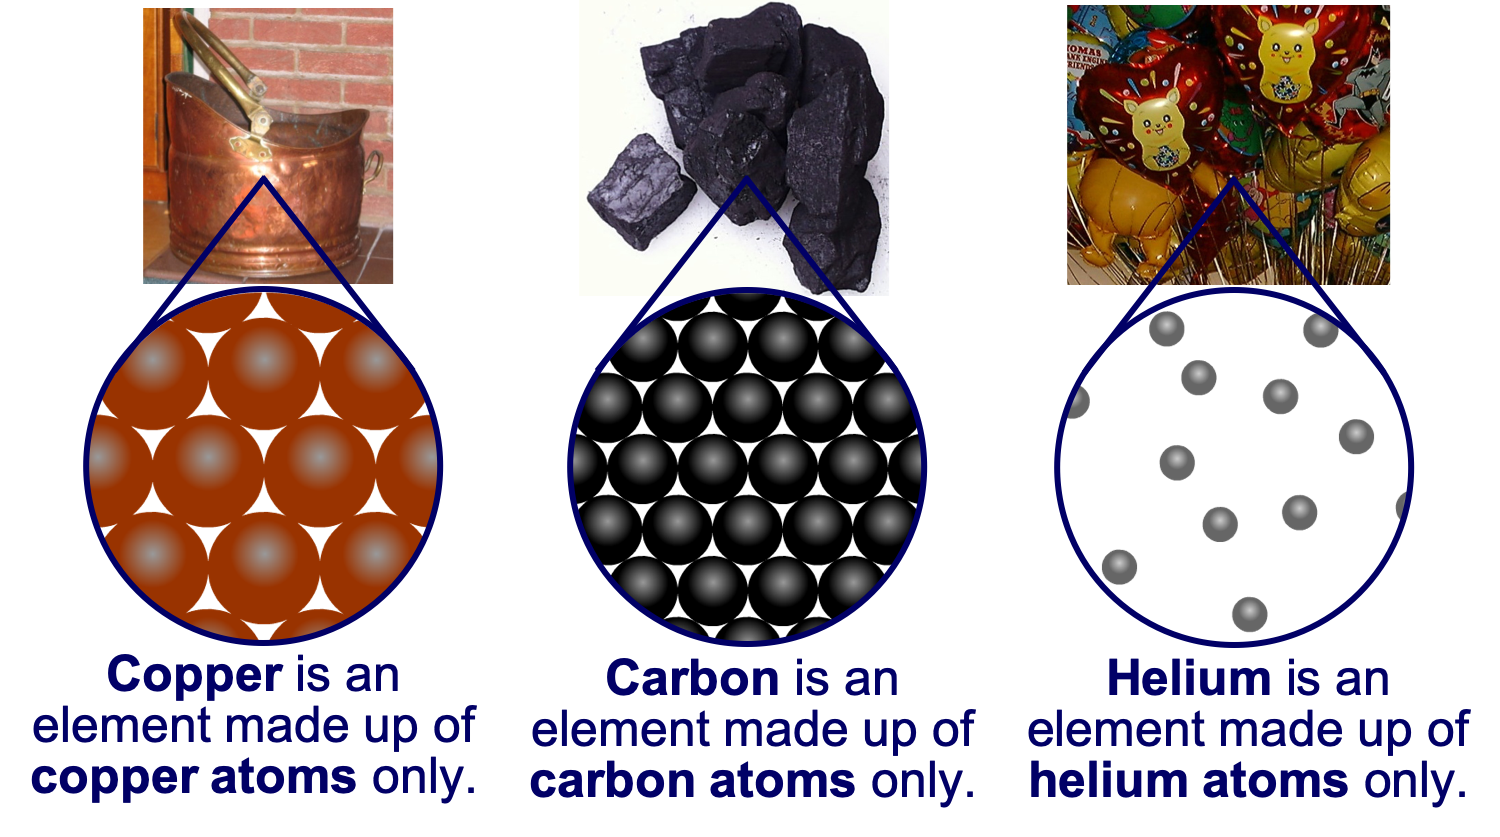
\includegraphics[width=0.9\linewidth]{elements.png}
	\end{center}
\end{wrapfigure}

\textbf{Pātai:} What makes the elements different from each other?\\
\vspace{2cm}

\subsection{Ngohe: Draw a labelled diagram of a lithium atom}

\newpage
\subsection{The Rutherford Model}

\begin{wrapfigure}[8]{r}{0.3\textwidth}
	\vspace{-1cm}
	\centering
	% Source: https://en.wikipedia.org/wiki/Rutherford_model
	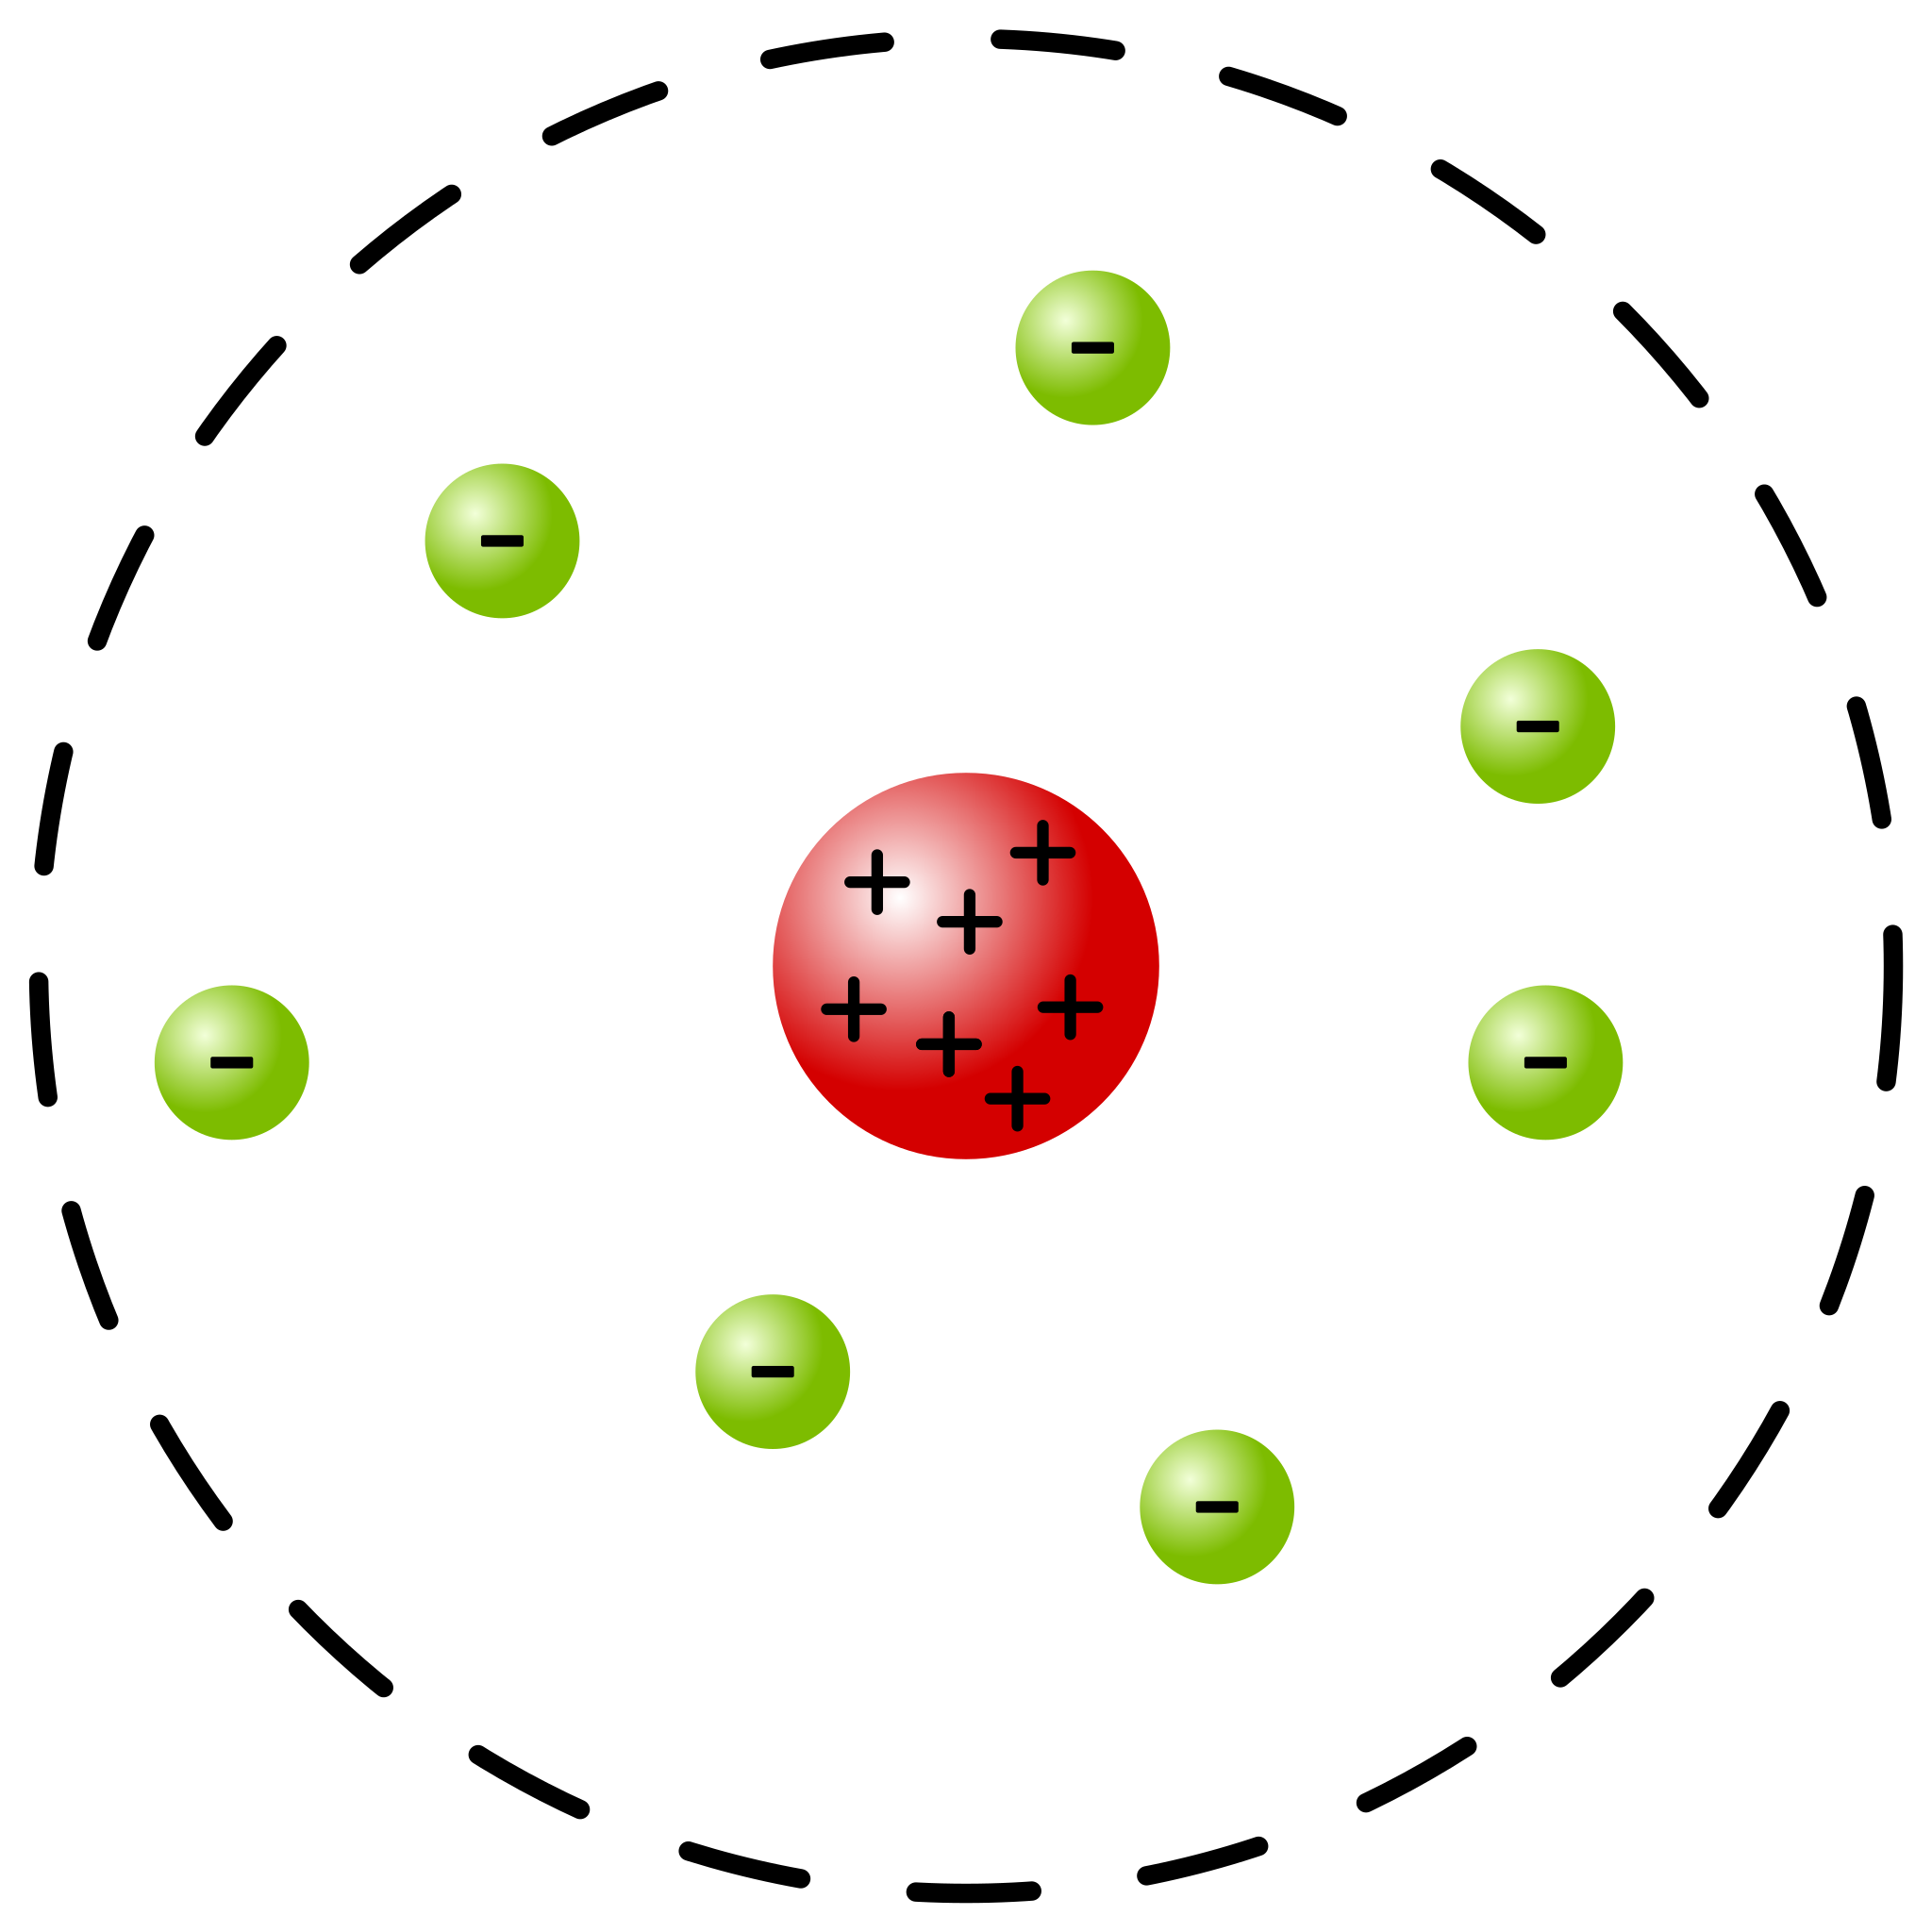
\includegraphics[width=0.9\linewidth]{rutherford-model.png}
\end{wrapfigure}

What you have drawn is the Rutherford Model of the atom. This model is the most common one we see in school today because it has very strong predictive powers. It is also very valuable because it allows to easily visualise things like \textit{ions} and \textit{isotopes} and how some chemical bonding works.

The central region is called the \fillinunderline{nucleus}. It is made of \fillinunderline{protons} and \fillinunderline{neutrons} which are strongly bound together by the \fillinspace{nuclear force}. Together we call protons and neutrons \fillinunderline{nucleons}, as they exist in the nucleus.

Electrons are constantly moving around the nucleus in a probabilistic way. This means that they do not have fixed orbits like the planets, but instead exist in a \text{probability cloud}. The size of the nucleus compared to the whole atom is very small, but it contains $>99.95\%$ of the mass because electrons are very light.

Protons have a \fillinunderline{positive} charge, electrons have a \fillinunderline{negative} charge, and neutrons have \fillinunderline{no} charge. Protons and electrons have an equal but opposite sized charge despite their very different masses.

\section{Atomic and Mass Numbers}
The number of protons in an atom (i.e. the atomic number) defines which type of atom it is. For example, and atom that has six protons MUST be a \fillinunderline{carbon} atom, and cannot be any other.

\begin{itemize}
	\item \textbf{Atomic number}: \fillinspace{The number of protons}
	\item \textbf{Mass number}: \fillinspace{The number of protons + neutrons}
\end{itemize}

\subsection{Ngohe: Reading the Periodic Table}

\renewcommand{\arraystretch}{2}
\begin{table}[hb]
\centering
\begin{tabular}{|l|l|l|l|l|l|l|}
\cline{2-7}
\hline
                   & \textbf{Protons}  & \textbf{Electrons}  & \textbf{Neutrons} & \textbf{Nucleons} & \bfseries{\makecell{Atomic \\ \#}} & \bfseries{\makecell{Mass \\ \#}} \\ \hline
\textbf{Oxygen}    & \fillinspace{8}   & \fillinspace{8}     & \fillinspace{8}   & \fillinspace{16}  & \fillinspace{8}                       &                                     \\ \hline
\textbf{Sodium}    & \fillinspace{11}  & \fillinspace{11}    & \fillinspace{12}  & \fillinspace{23}  & \fillinspace{11}                      &                                     \\ \hline
\textbf{Aluminium} & \fillinspace{13}  & \fillinspace{13}    & \fillinspace{14}  & \fillinspace{27}  & \fillinspace{13}                      &                                     \\ \hline
\textbf{Copper}    & \fillinspace{29}  & \fillinspace{29}    & \fillinspace{35}  & \fillinspace{64}  & \fillinspace{29}                      &                                     \\ \hline
\end{tabular}
\end{table}

\newpage
\section{Ions}

\begin{wrapfigure}[7]{r}{0.5\textwidth}
	\vspace{-1cm}
	\begin{center}
		% Source: https://static-cdn.imageservice.cloud/3528258/igcse-chemistry-2017-140-draw-dot-and-cross-diagrams-to-show-the.jpg
		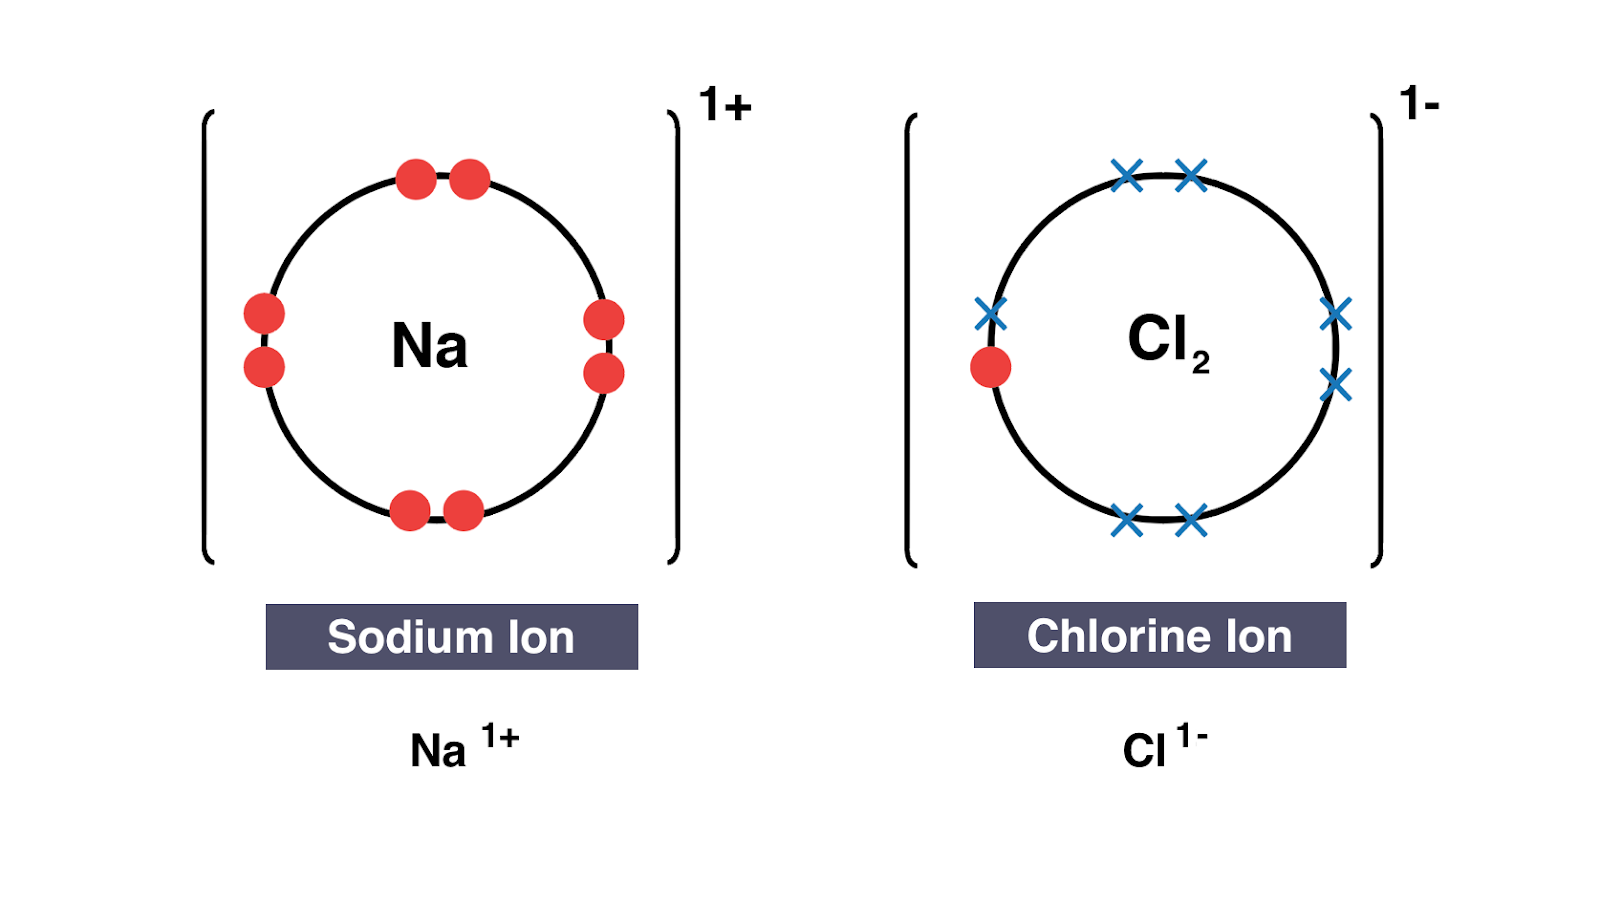
\includegraphics[width=0.9\linewidth]{ion.png}
	\end{center}
\end{wrapfigure}

An atom is a neutral particle, having equal number of protons and electrons (recall: they have opposite but equal size electric charges). However, an atom may lose or gain one or more electrons during a reaction. This causes them to gain a \textit{net charge}. When an atom has a charge it is called an \fillinunderline{ion}.
Positively charged ions are called \fillinunderline{cations} and negatively charged ions are called \fillinunderline{anions}.

\section{Isotopes}

\begin{wrapfigure}[11]{l}{0.4\textwidth}
	\vspace{-1cm}
	\begin{center}
		% Source: https://isotopes.gov/isotope-basics
		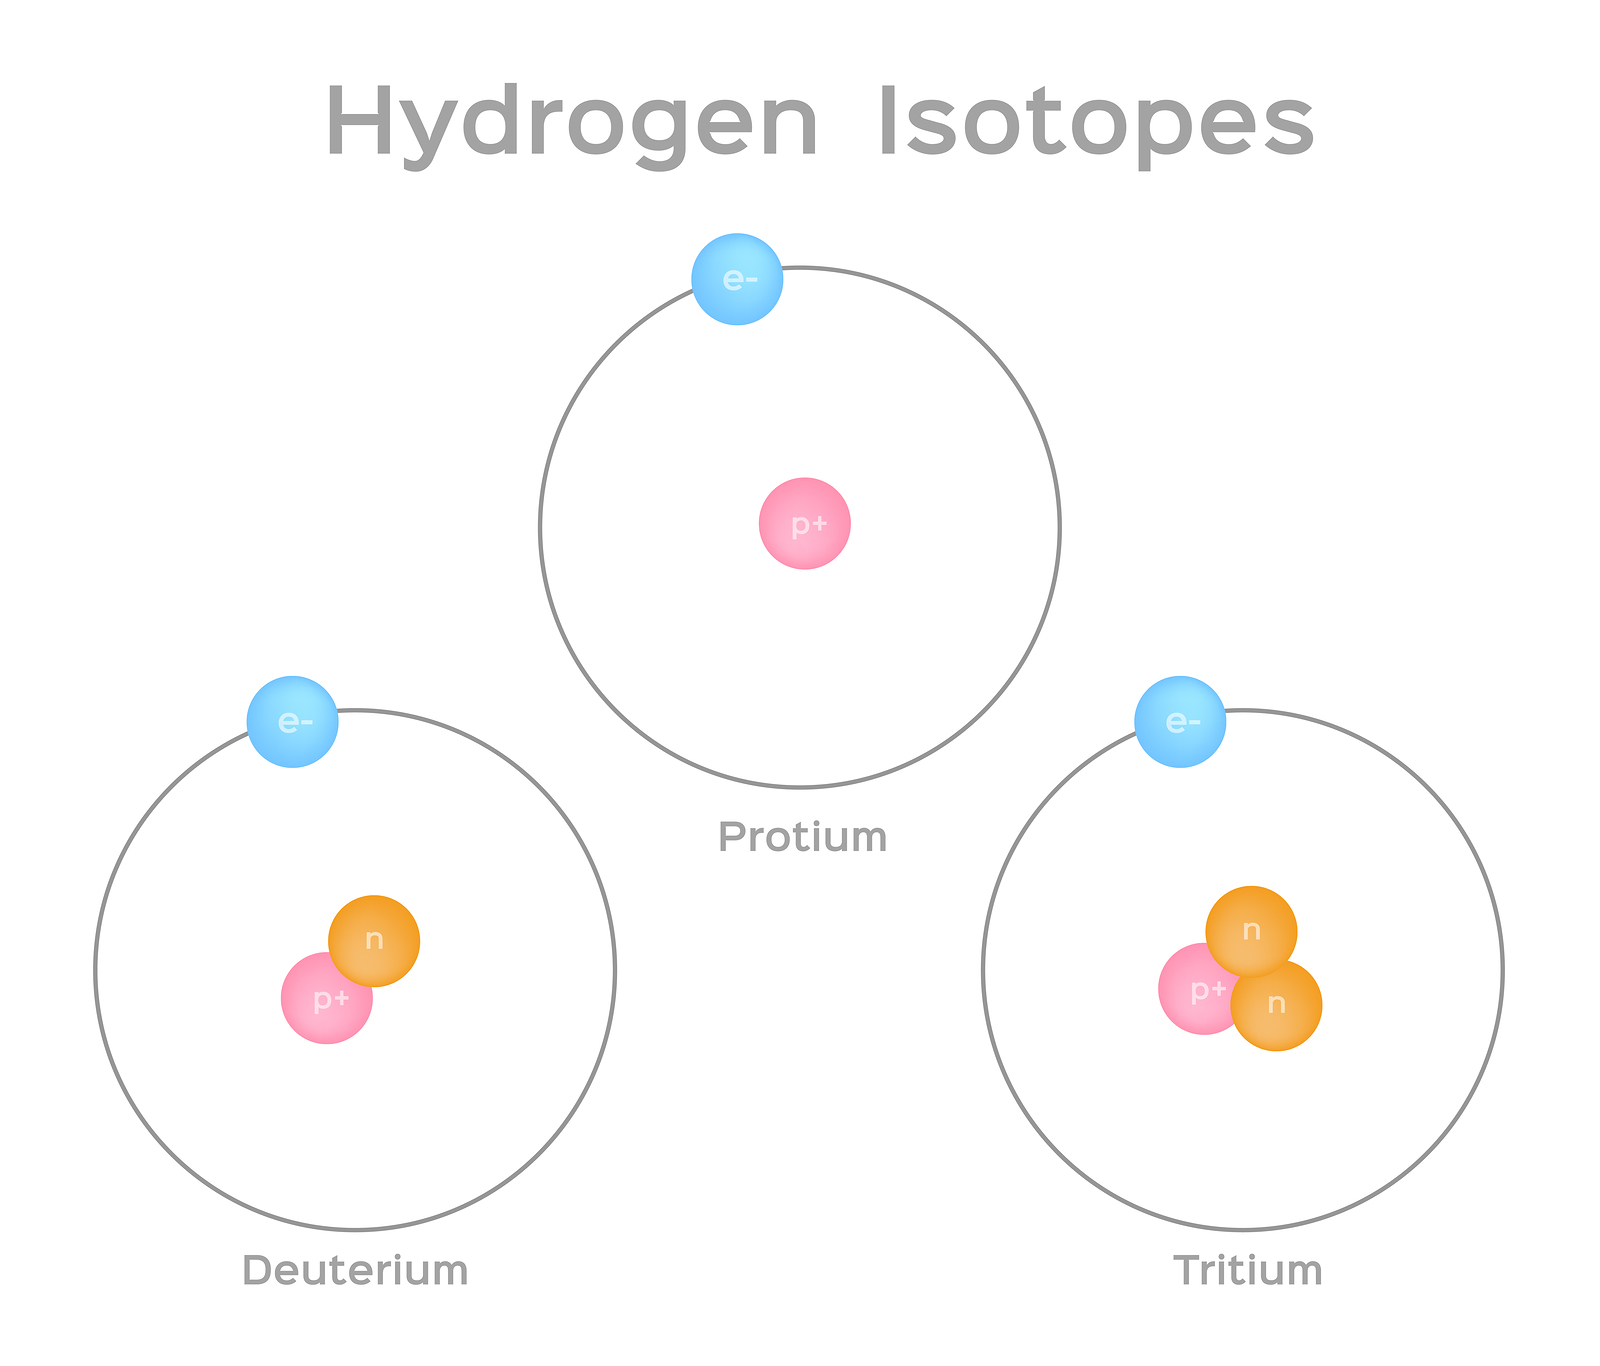
\includegraphics[width=0.9\linewidth]{isotopes.jpg}
	\end{center}
\end{wrapfigure}

An isotope is an atom with the same number of protons (same element), but with a different number of neutrons. This means that the \textit{atomic number} is the same, but that the \textit{mass number} is different.

This is why some periodic tables show a mass number with lots of decimal places, \underline{it is an average of the different isotopes}.

Some isotopes are stable, while others like Carbon-14 is radioactive and will decay over time. Carbon-14 can be used to find the age of organic matter. They do this by looking at the ratio of Carbon-14 compared to the other isotopes.

\subsection{Ngohe: Carbon Isotopes}

For Carbon-12, Carbon-13 and Carbon-14, complete the table below.

\begin{table}[ht]
\centering
\begin{tabular}{l|l|l|l|l|l|l|}
\cline{2-7}
                                         & \textbf{Protons} & \textbf{Electrons} & \textbf{Neutrons} & \textbf{Nucleons} & \bfseries{\makecell{Atomic \\ \#}} & \bfseries{\makecell{Mass \\ \#}} \\ \hline
\multicolumn{1}{|l|}{\textbf{Carbon-12}} & \fillinspace{6}  & \fillinspace{6}    & \fillinspace{6}   & \fillinspace{12}  & \fillinspace{6}                    & \fillinspace{12}                 \\ \hline
\multicolumn{1}{|l|}{\textbf{Carbon-13}} & \fillinspace{6}  & \fillinspace{6}    & \fillinspace{7}   & \fillinspace{13}  & \fillinspace{6}                    & \fillinspace{13}                 \\ \hline
\multicolumn{1}{|l|}{\textbf{Carbon-14}} & \fillinspace{6}  & \fillinspace{6}    & \fillinspace{8}   & \fillinspace{14}  & \fillinspace{6}                    & \fillinspace{14}                 \\ \hline
\end{tabular}
\end{table}

\section{Whakawai: Atomic Structure}

Atoms are made of a central dense part called the \fillinunderline{nucleus} surrounded by a moving cloud of \fillinunderline{electrons}. The particles in the central region are called nucleons and are either protons or \fillinunderline{neutrons}. The charge on protons is \fillinunderline{positive}.

The nucleons are attracted strongly to each other by a force called the \fillinunderline{nuclear} force. The protons however, repel each other, because they have similar charges. This repulsion force between the protons is an \fillinunderline{electrostatic} force. As a result of these forces in the nucleus, most nuclei are stable. However, if nuclei are disrupted by nuclear reactions enormous amounts of \fillinunderline{energy} may be released. The reason for this is that the \fillinunderline{forces} in the nucleus are very strong.

The atomic number is the number of \fillinunderline{protons} in the nucleus of an atom. The mass number is the number of \fillinunderline{protons} and \fillinunderline{neutrons} in the nucleus of an atom. Isotopes of an element will always have the same \fillinunderline{atomic} number but different \fillinunderline{mass} numbers.


% =========================
%  2. Atomic Structure
% =========================
\newpage
\chapter{Atomic Structure}

\noindent\textbf{Learning Outcomes}
\begin{nwa}
	\item Understand the history and process of how we formulated the current atomic model
\end{nwa}

\noindent\href{https://youtu.be/xazQRcSCRaY}{Introductory Video: https://youtu.be/xazQRcSCRaY}

\section{The Greeks}
As mentioned earlier, Aristotle and the Greeks in 450BC thought that everything was made of water, earth, air and fire. Some years later, another Greek philosopher Democritus came up with the idea of some indivisible piece of matter - a fundamental building block. He did not know what it was, but theorised that one should exist. He called these pieces of matter \textit{atomos (Latin: indivisible)}.

\section{John Dalton (1766 - 1844)}

\begin{wrapfigure}[6]{r}{0.25\textwidth}
	\vspace{-1cm}
	\begin{center}
		% Source: https://isotopes.gov/isotope-basics
		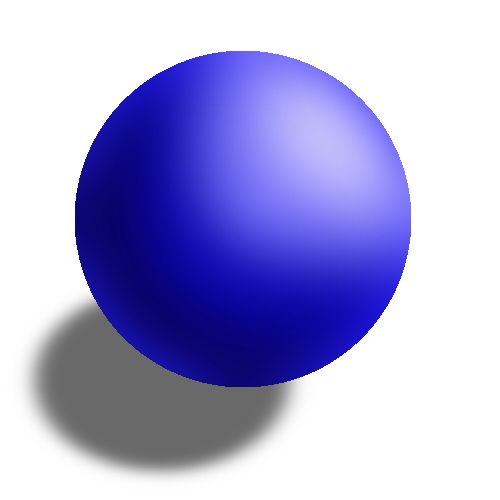
\includegraphics[width=0.9\linewidth]{dalton-model.jpg}
		\caption{Dalton's ball theory of the atom.}
	\end{center}
\end{wrapfigure}

John Dalton was an English chemist who introduced \textit{atomic theory} into chemistry. There is some debate about where he got his theory, but the main points he developed were:

\begin{itemize}
    \item Elements are made of extremely small particles called atoms
    \item Atoms of a given element are \fillinunderline{identical in size}, \fillinunderline{mass}, and other properties
    \item Atoms cannot be \fillinunderline{subdivided, created or destroyed}.
    \item Atoms of different elements combine in simple whole-number ratios to form chemical compounds. E.g. $MgCl_{c}$.
    \item In chemical reactions, atoms are combined, separated or rearranged.
\end{itemize}

He was not able to ascertain the weight of any elements, but did attempt to order them by \textit{relative weight}. It was with John Dalton when \textit{atomos} from the Greeks became \textit{atoms}.

\section{Joseph Thomson (1856–1940)}\

\begin{wrapfigure}[12]{r}{0.25\textwidth}
	\vspace{-1cm}
	\begin{center}
		% https://www.universetoday.com/38326/plum-pudding-model/
		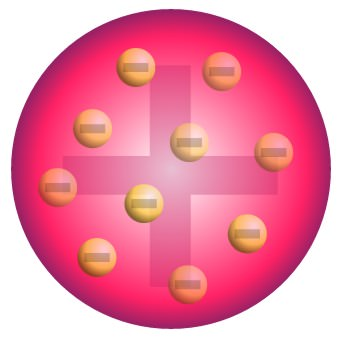
\includegraphics[width=0.9\linewidth]{thomson-model.jpg}
		\caption{Thomson's Plum Pudding theory of the atom.}
	\end{center}
\end{wrapfigure}

Joseph Thomson was a British physicist who did a lot of work with cathode rays (\fillinunderline{streams of electrons}) and who was awarded the Nobel Laureate in Physics for discovering the electron. This was the first subatomic particle to be discovered! He is also credited with finding the first scientific evidence of \fillinunderline{isotopes}.

At the time of his research he was not originally aware that cathode rays were streams of "electrons". He only knew that they were negatively charged and had \fillinunderline{a very small mass}. He hypothesised that the electrons were emitted from the atoms inside the cathode ray tube, and thus concluded \fillinunderline{that atoms were in fact divisible}.

If the electrons were inside the atoms, and an atom was neutral, the electrons would have to be evenly distributed throughout, and the atom itself made of some positive material.

\section{Ernest Rutherford (1871-1937)}

\begin{wrapfigure}[10]{r}{0.2\textwidth}
	\vspace{-1cm}
	\begin{center}
		% Source: https://en.wikipedia.org/wiki/Rutherford_model
		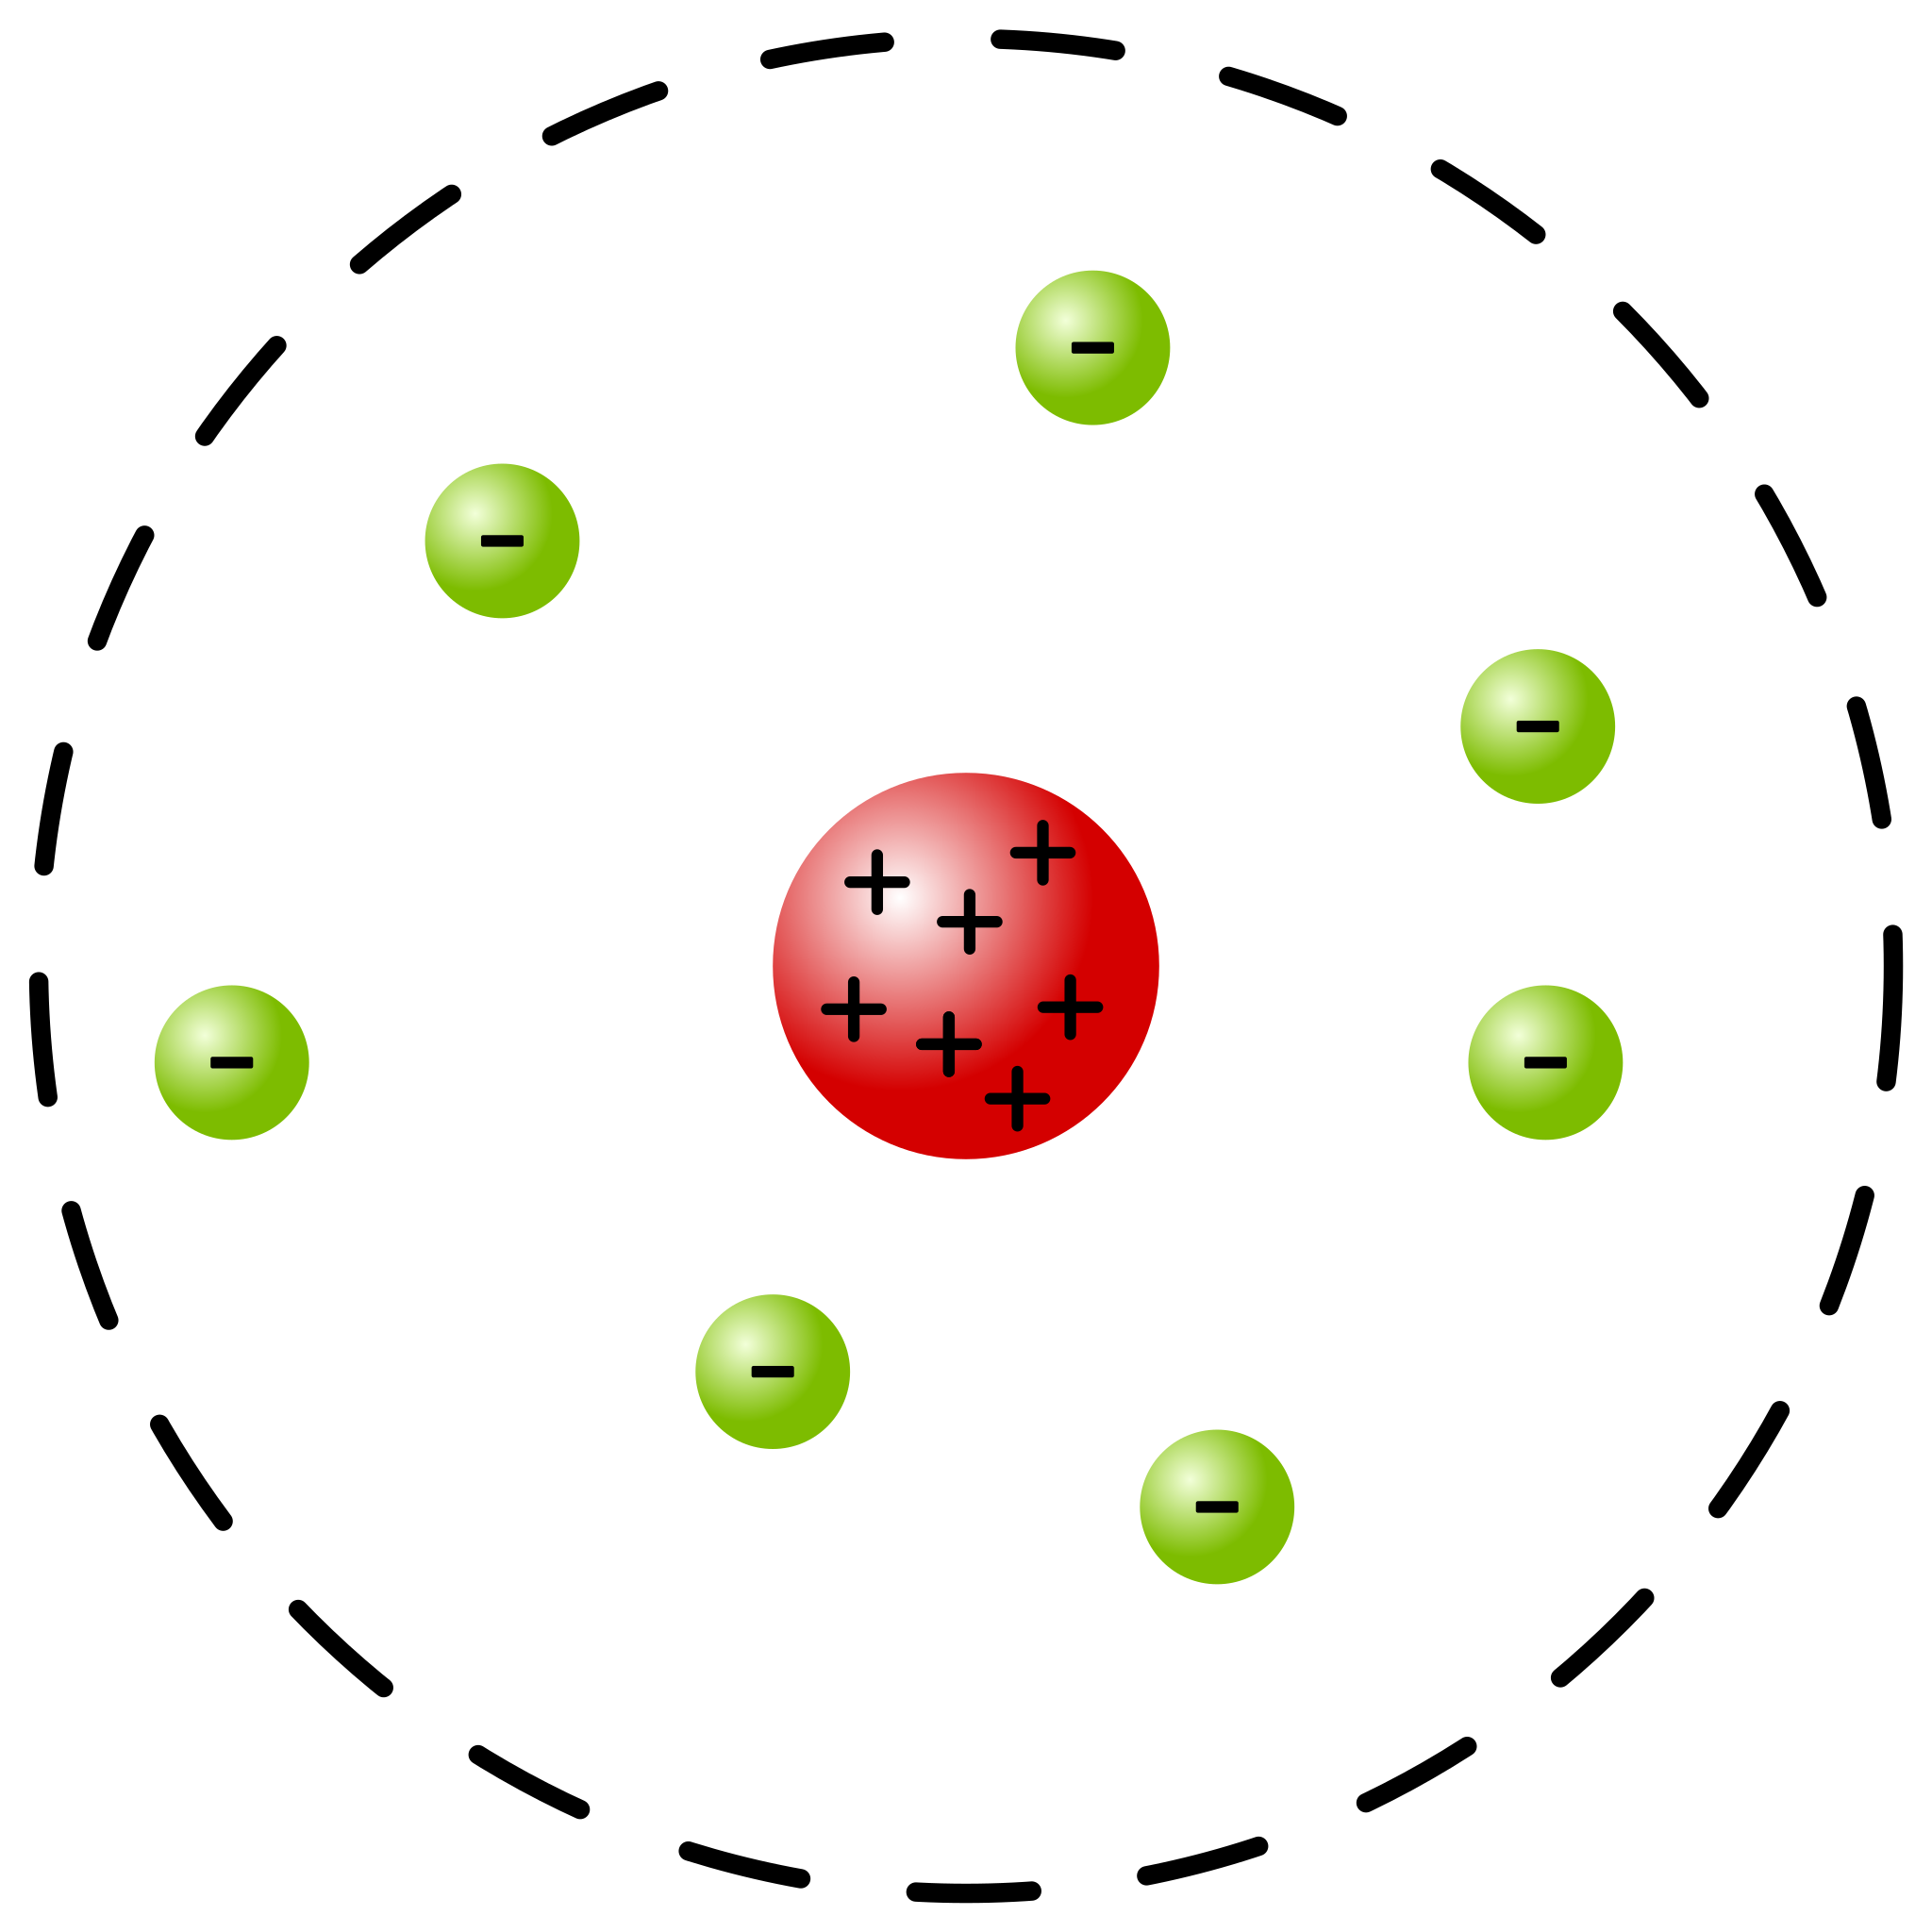
\includegraphics[width=0.9\linewidth]{rutherford-model.png}
		\caption{Rutherford's Model of the Atom}
	\end{center}
\end{wrapfigure}

Ernest Rutherford is a New Zealand-born British Physicist credited as the father of nuclear physics. He was the discoverer of the concept of \fillinunderline{radioactive half-life}, and was awarded the Nobel Prize in Chemistry for his work into the disintegration of the elements (\fillinunderline{radioactivity}).

His work on the atom revolved around something called \fillinunderline{The Gold Foil Experiment} where he fired alpha particles (\fillinunderline{helium nuclei}) at a sheet of thin gold foil. By analysing the scatter pattern of the alpha particles he was able to determine that there is a positive nucleus in the centre of the atom, and that the electrons should orbit around the outside. \textit{Notice that at this point we still have not discovered the neutron}.

\newpage
\section{The Gold Foil Experiment}

\noindent\href{https://www.youtube.com/watch?v=1EdTw4I6L0U}{Introductory Video: https://www.youtube.com/watch?v=1EdTw4I6L0U}

\begin{figure}[ht]
	\centering
	\begin{subfigure}{0.5\textwidth}
		\centering
		% Source: https://cnx.org/contents/LxK68dbM@4.9:67SLu9dU@4/Structure-of-an-Atom
		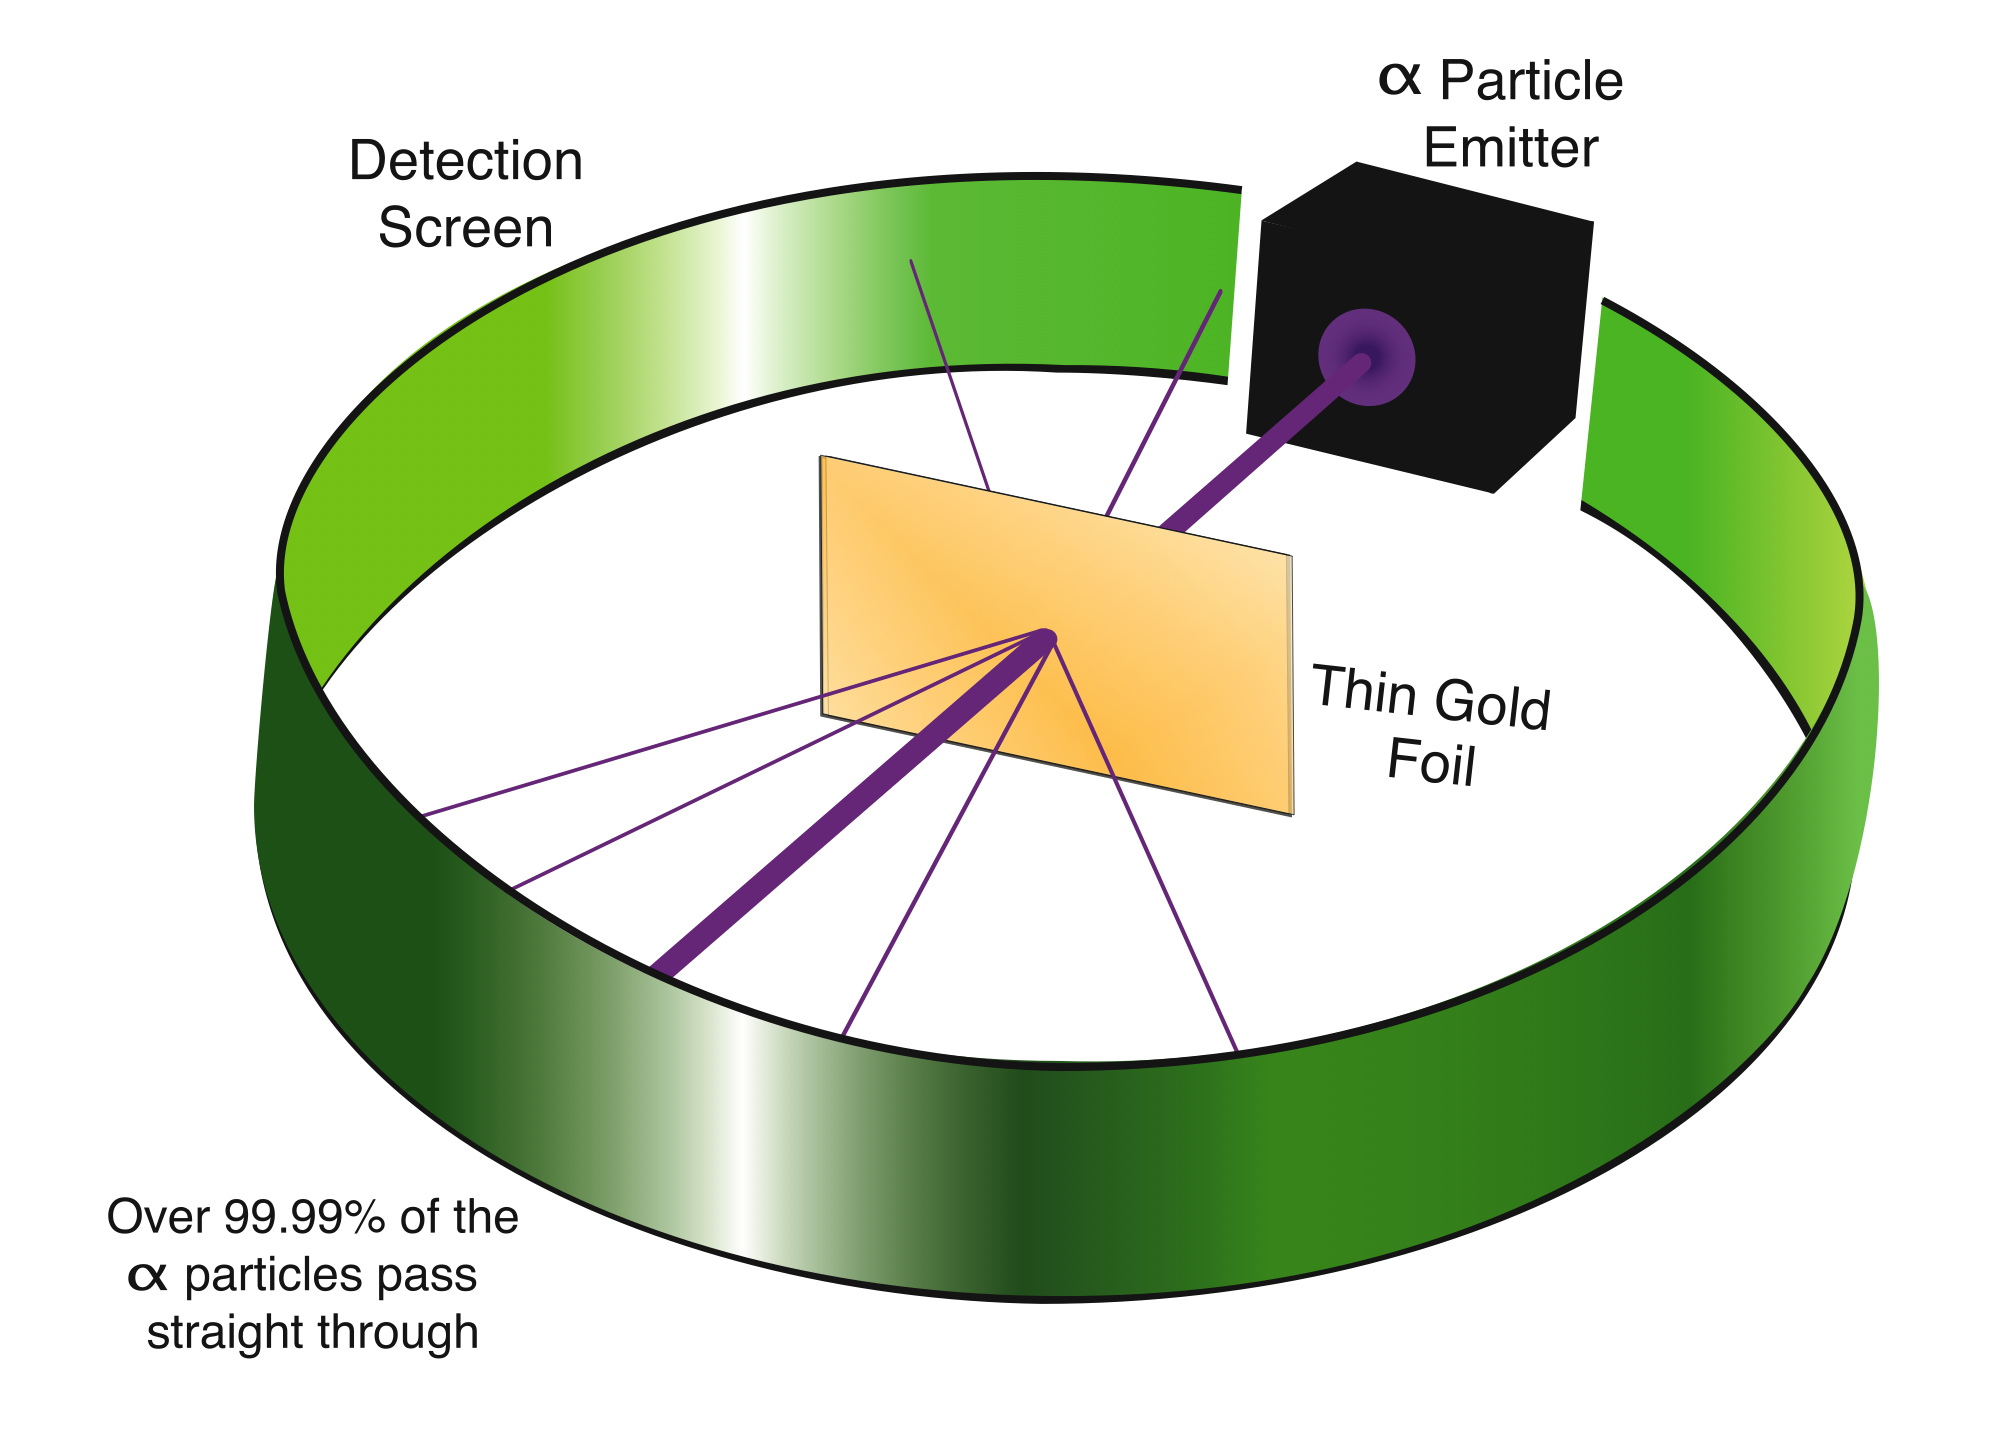
\includegraphics[width=\linewidth]{gold-foil-experiment.png}
		% \caption{Rutherford's Gold Foil Experiment}
	\end{subfigure}%
	\begin{subfigure}{.5\textwidth}
		\centering
		% Source: https://cnx.org/contents/LxK68dbM@4.9:67SLu9dU@4/Structure-of-an-Atom
		\ifthenelse{\boolean{@answer}}
			{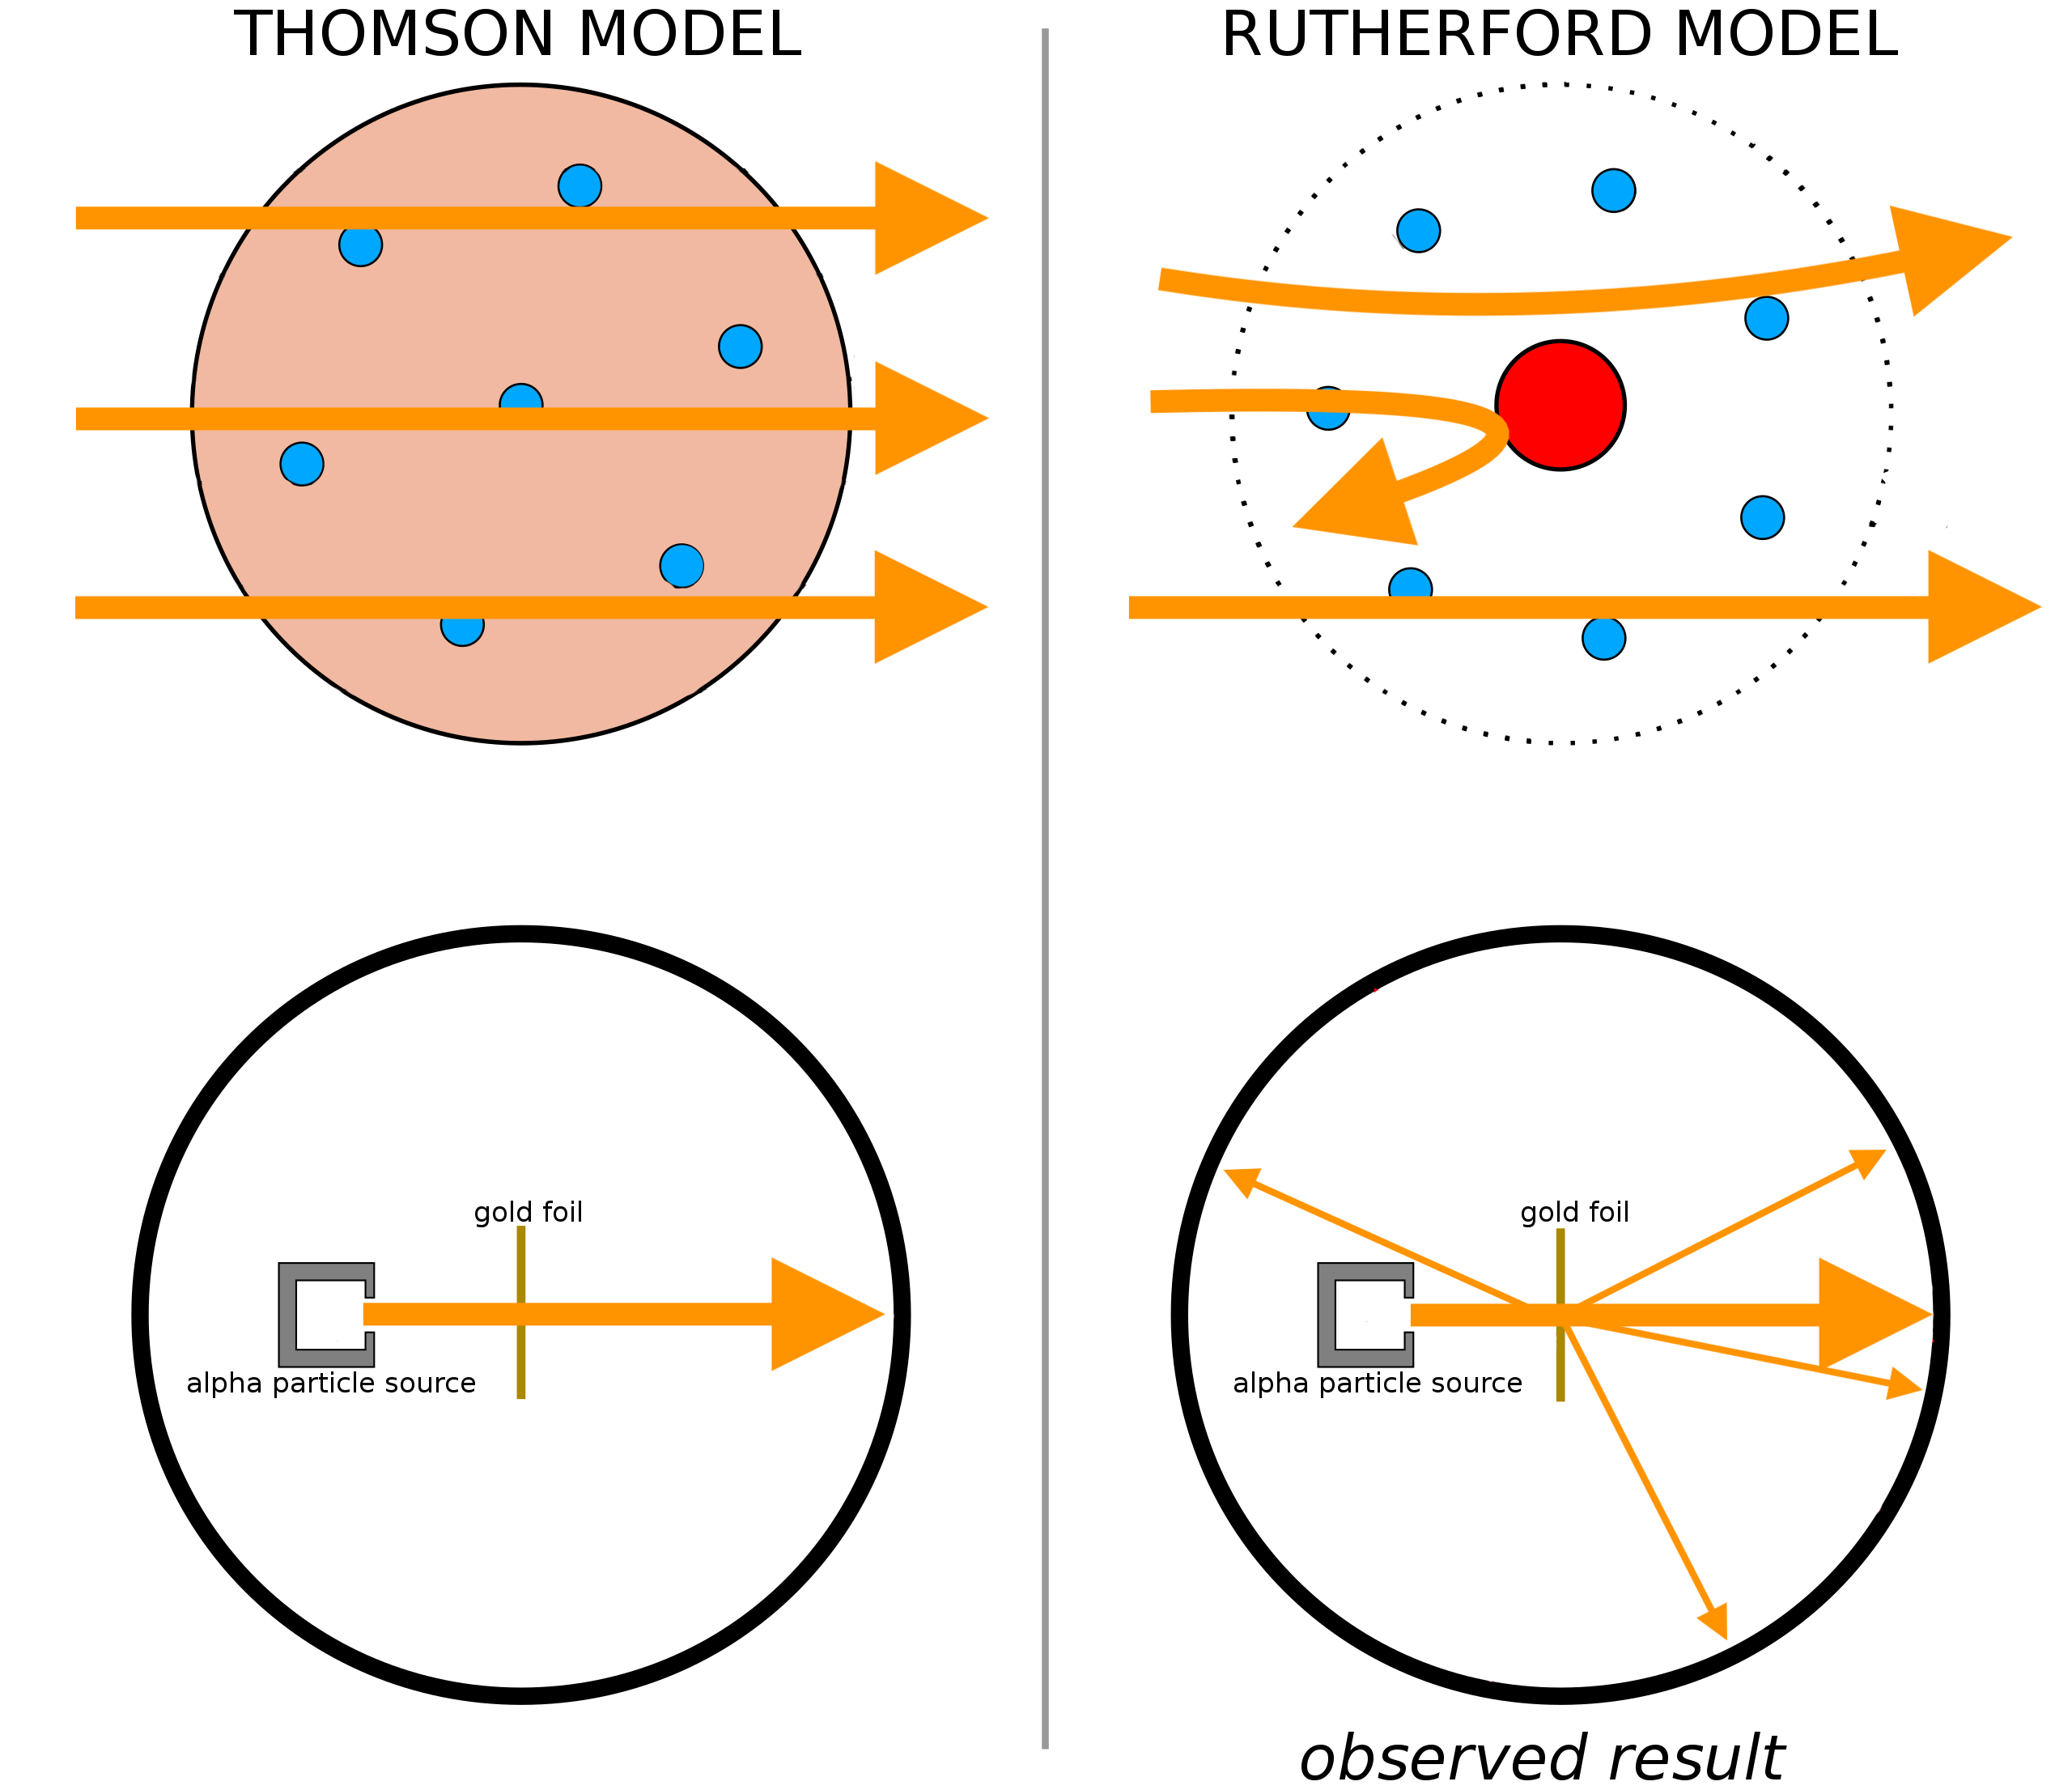
\includegraphics[width=\linewidth]{assets/atom-model-comparison-answer.png}}
			{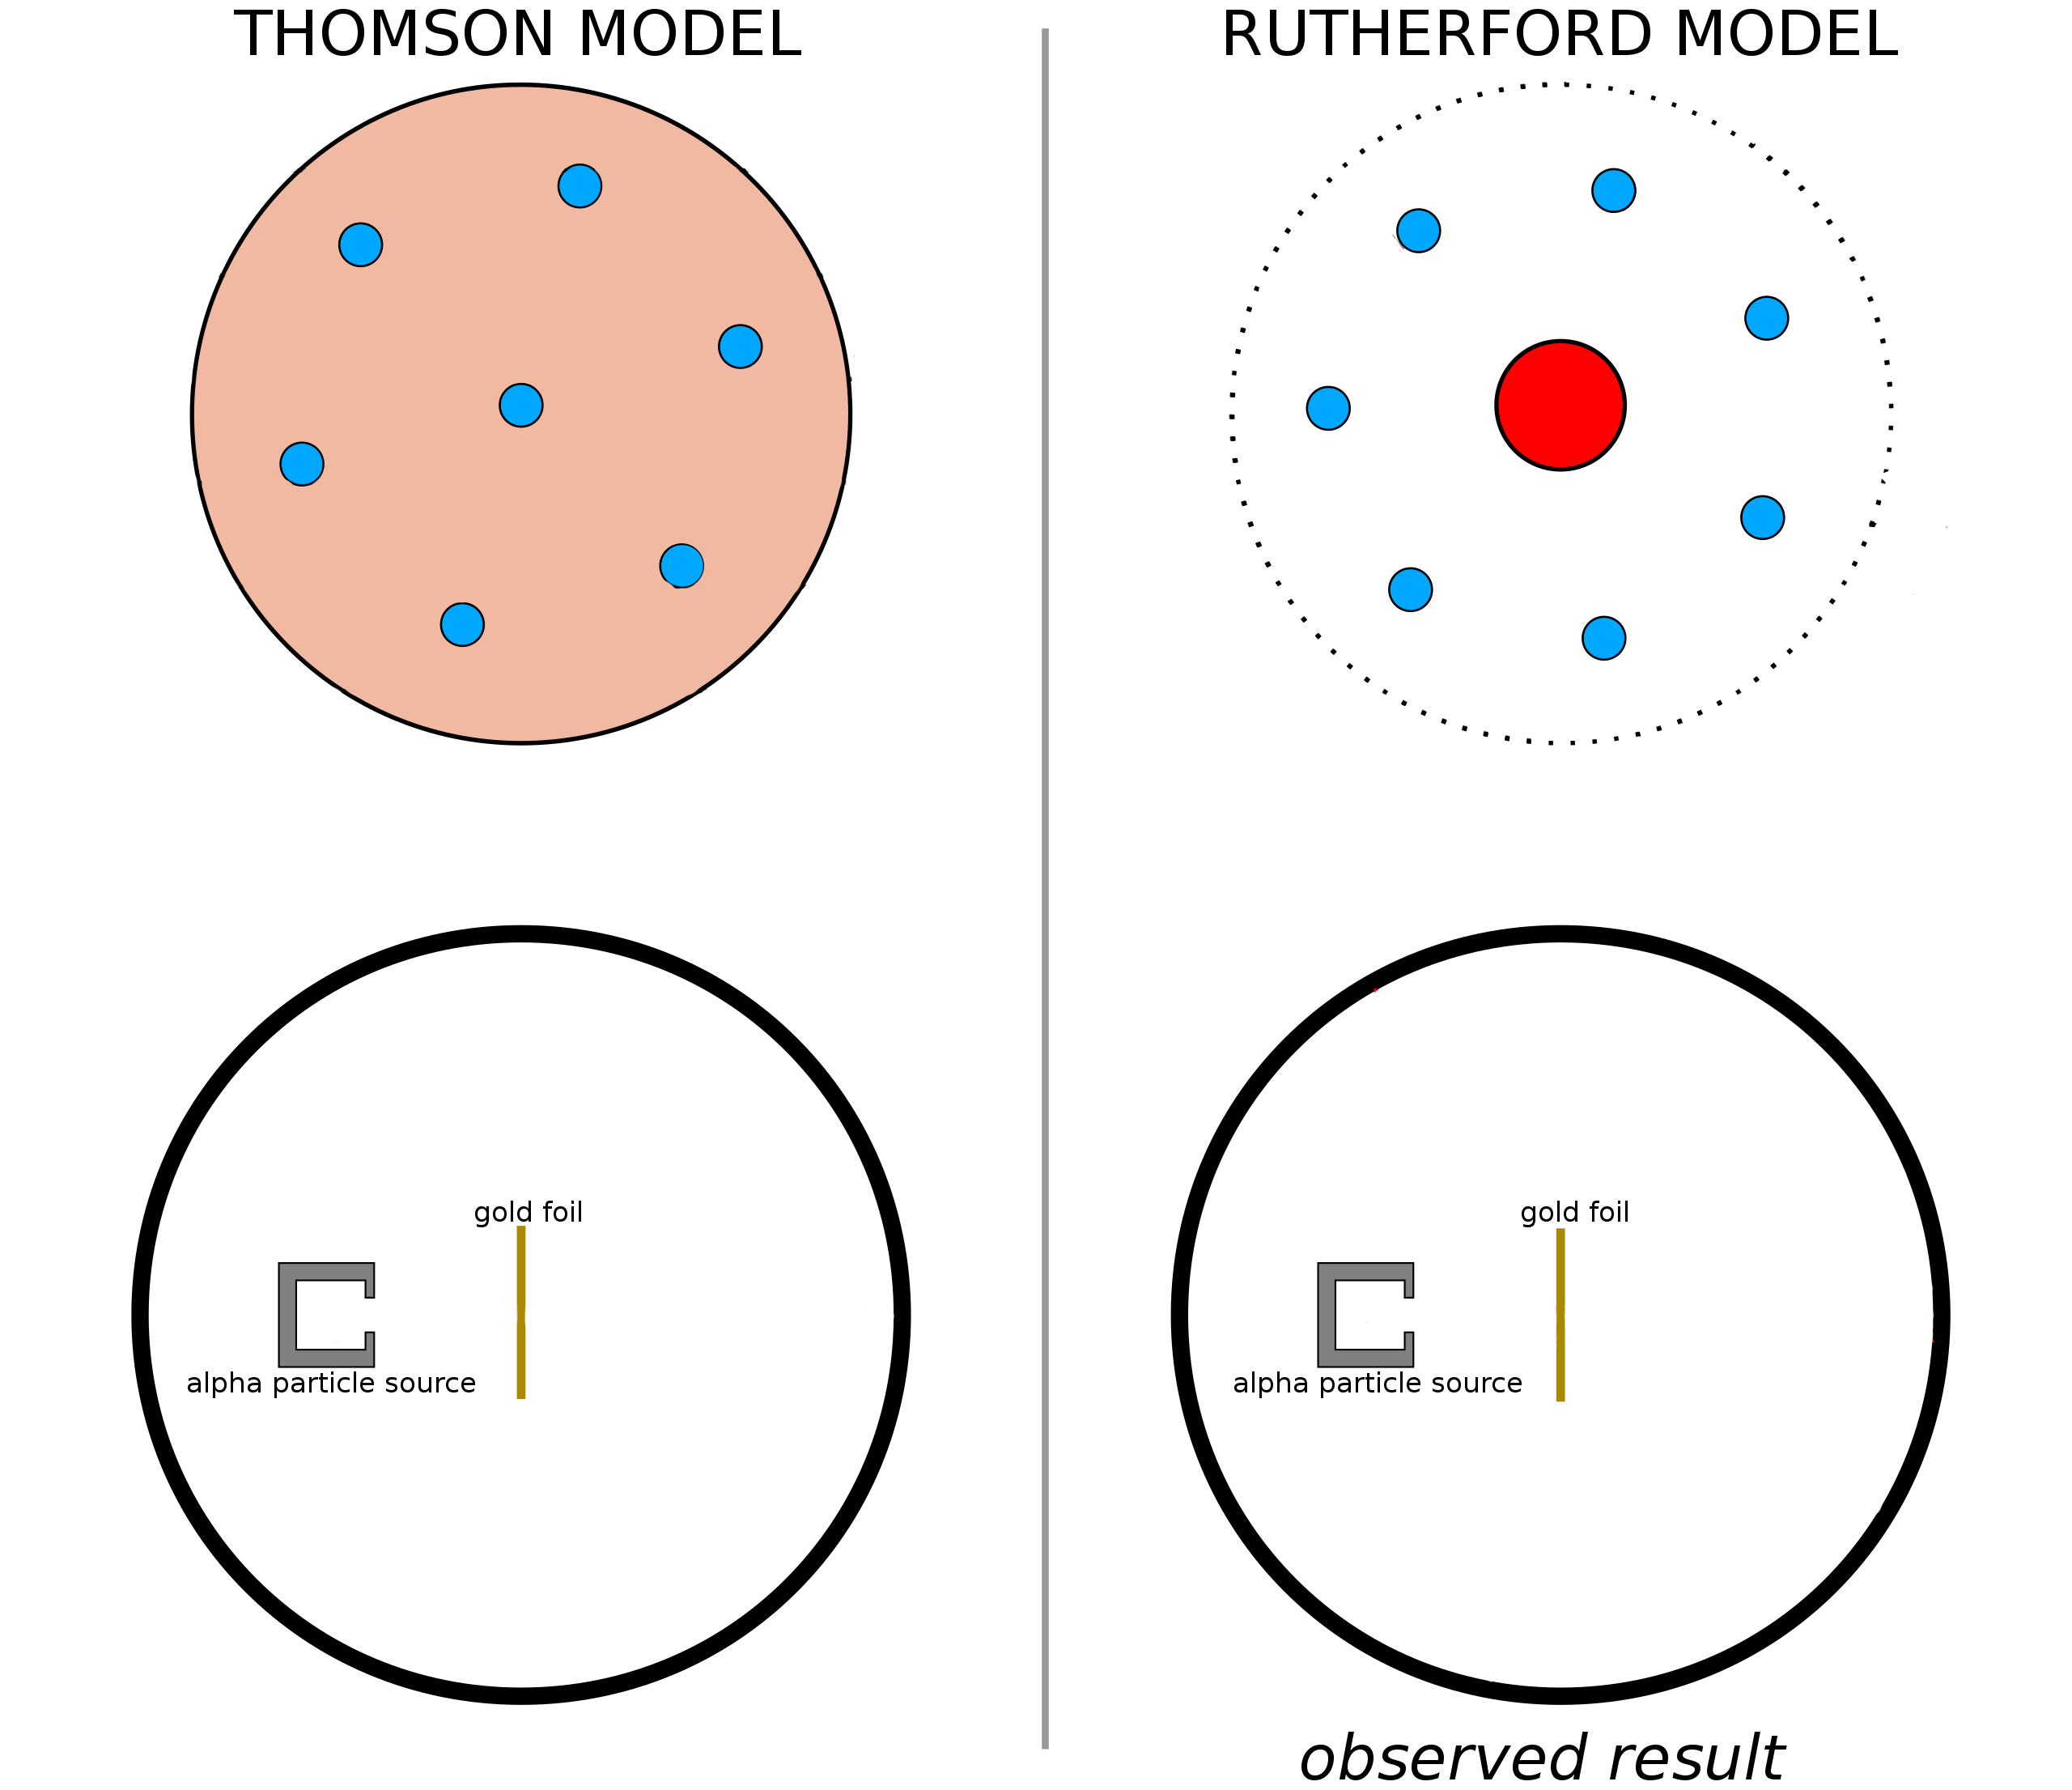
\includegraphics[width=\linewidth]{assets/atom-model-comparison.png}}
	\end{subfigure}
\end{figure}

\begin{enumerate}
	\item \textbf{Observation 1}: Most alpha particles were found to go straight through the foil.\\
	\textbf{Conclusion:}
	\fillinspace{The atom consists of mostly empty space.}
	\StudentVSpace{1cm}

	\item \textbf{Observation 2}: Some alpha particles experienced a small angle of deflection. \\
	\textbf{Conclusion:}
	\fillinspace{There is a positively charged mass within the nucleus that can deflect particles at a small angle if they pass nearby.}
	\StudentVSpace{1cm}
	
	\item \textbf{Observation 3}: Very few alpha particles were deflected. \\
	\textbf{Conclusion:} \fillinspace{The charged mass has a very small volume.}
	\StudentVSpace{1cm}
	
	\item \textbf{Observation 4}: Some particles were deflected at a very large angle. \\
	\textbf{Conclusion:} \fillinspace{The charged mass is very dense.}
	\StudentVSpace{1cm}
	
	\item Explain why the gold foil experiment had to be carried out in a vacuum.
	\fillinspace{So that the path of the alpha particles could not be affected by air molecules. This way we can be sure that any deviations are due to the gold atoms.}
	\StudentVSpace{2cm}
	
	\item Explain why it was necessary for the gold foil to be a few atoms thick.
	\fillinspace{So that the alpha particles are able to pass through. Thicker gold would stop all alpha particles and not allow any measurements to be made.}
	\StudentVSpace{2cm}
	
	\item Describe one way in which Thomson's and Rutherford's models of the atom were similar.
	\fillinspace{They both have positive and negative parts.\\The negative parts are small.}
	\StudentVSpace{1.5cm}
	
	\item Describe the key difference between Thomson's and Rutherford's model of the atom.
	\fillinspace{
	The positive matter is condensed in the nucleus for Rutherford, and spread out for Thompson.\\
	There exists very little mass around the nucleus for Rutherford.
	}
	\StudentVSpace{1.5cm}
	
	\item In front of the alpha emitter is a lead screen with a narrow slit cut in it. What function does this lead screen serve?
	\fillinspace{It stops all alpha particles except those moving in a very straight line towards the gold foil, from passing out of the box. Therefore eliminating any false detections on an angle.}
	\StudentVSpace{2cm}
	
	\item What would Rutherford have seen if Thomson's model of the atom was correct?
	\fillinspace{There would not have been any deviation of alpha particle path due to the lack of dense positive material.}
	\StudentVSpace{2cm}
	
	\item What would have been observed if Rutherford used a beta emitter instead of an alpha emitter?
	\fillinspace{The electrons will be more easily scattered because they have a low mass.}
	\StudentVSpace{2cm}
\end{enumerate}

% =========================
%  3. Nuclear Decay
% =========================
\newpage
\chapter{Nuclear Decay}

\noindent\textbf{Learning Outcomes}
\begin{nwa}
	\item Describe alpha radioactive decay
	\item Describe beta radioactive decay
	\item Describe gamma radioactive decay
\end{nwa}

\noindent\href{https://youtu.be/UtZw9jfIxXM}{Introductory Video: https://youtu.be/UtZw9jfIxXM}

\section{Pātai: What is a nuclear reaction?}

\begin{itemize}
	\item It \textbf{is not} a physical reaction (e.g. changing state)
	\item It \textbf{is not} a chemical reaction (e.g. forming ionic compounds)
	\item It \textbf{is} a reaction where: \fillinspace{the nucleus of an atom changes}
\end{itemize}

\noindent There are three types of nuclear reactions that we are interested in for this topic:

\begin{itemize}
	\item \fillinspace{\textbf{Radioactive Decay (alpha, beta, gamma)}}
	\item \fillinspace{Nuclear Fission}
	\item \fillinspace{Nuclear Fusion}
\end{itemize}

\section{Why Nuclear Decay Occurs}

\begin{wrapfigure}{r}{0.5\linewidth}
	\centering
	% Source: https://en.wikipedia.org/wiki/Radioactive_decay
	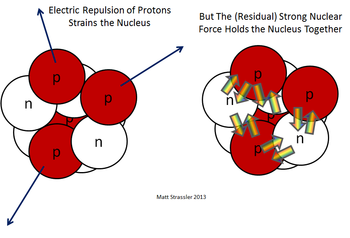
\includegraphics[width=0.9\linewidth]{assets/nucleus-force-comparison.png}
	% \caption{The neutron added to the nucleus makes it unstable and decay occurs.}
\end{wrapfigure}

Inside the nucleus are the protons and neutrons. The neutrons do not carry an electric charge, so do not interact electrically. The protons, however, carry a positive charge. We know that like charges repel, so \textit{why does the nuclear not fall apart?}

It turns out that when nucleons get close enough another force comes into effect: the \fillinunderline{strong nuclear force}. This force glues the nucleons together. Nuclear decay occurs when the nucleus gets very large; either by having a large atomic number, or by being an isotope with a large number of neutrons.

Adding nucleons increases the volume of the nucleus, and thereby diluting the strong nuclear force. When the strong nuclear force is diluted such that the electrostatic force is now larger, the nucleus \fillinunderline{may split apart}. This is called radioactive decay!

Recall the Law of Conservation of Energy. Similar laws apply to nuclear equations and these four properties are also conserved:

\begin{itemize}
	\item \fillinspace{Energy}
	\item \fillinspace{Momentum (linear and angular)}
	\item \fillinspace{Electric and Magnetic Charge}
	\item \fillinspace{Nucleon (mass) Number}
\end{itemize}

\noindent\href{https://www.youtube.com/watch?v=TJgc28csgV0}{Video: https://www.youtube.com/watch?v=TJgc28csgV0}

\section{Ionizing Radiation}

Ionising means to have the ability to strip electrons from an atom/molecule. In some circumstances this can cause bonds to break - this can be bad in regards to cells and DNA. Heavy atoms like $\alpha$ particles may also simply break a molecule on impact (\fillinunderline{think $p=mv$}).

The ability to ionize is also characterised by having an electric charge. Neutral particles are less ionising. Low energy electromagnetic radiation is also not ionising. This is why your phone or microwave cannot harm you, but repeated x-rays can.

\begin{figure}[ht]
	\centering
	% Source: https://www.mirion.com/learning-center/radiation-safety-basics/what-is-radiation
	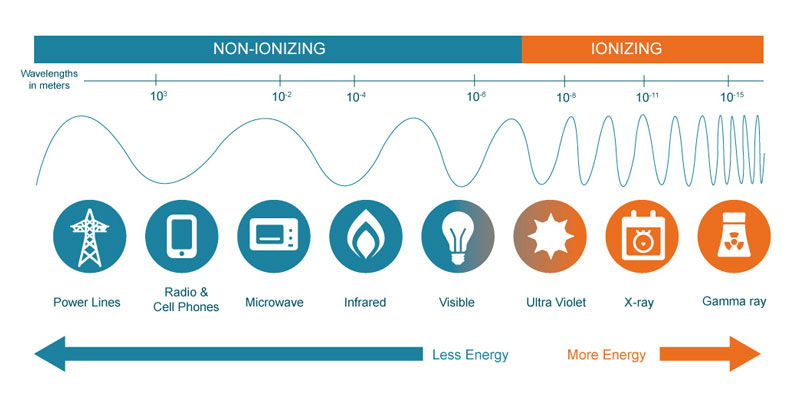
\includegraphics[width=0.9\linewidth]{assets/ionising-radiation.jpg}
\end{figure}

\section{Alpha Decay}

\begin{wrapfigure}[13]{r}{0.3\linewidth}
	\centering
	% Source: https://www.britannica.com/science/alpha-decay
	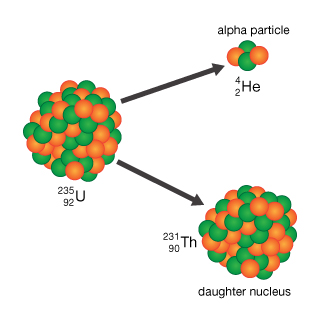
\includegraphics[width=0.9\linewidth]{alpha-decay.jpg}
	\caption{Alpha decay of a U-235 nucleus.}
\end{wrapfigure}

During alpha ($\alpha$) decay a particle is emitted from the nucleus. This particle is a \fillinunderline{helium nuclei}, also known as an alpha particle \fillinunderline{${}^{4}_{2}He^{2+}$}. It is positively charged because it contains just two neutrons and two protons.
It is slow moving (up to 10\% the speed of light) due to its relatively large mass. Its large mass means it can only move \fillinunderline{a few cm} through the atmosphere before being absorbed or \textit{redirected}. It also means that it is \fillinunderline{easy to protect against}. Conversely, the large mass (high momentum) means that it will do a lot of damage if it impacts organic matter like DNA. It is said to have \fillinunderline{the greatest ionising ability}

The majority of alpha emitters are the elements with atomic number greater than 83, although some other smaller nuclei also undergoing alpha emission.

\section{Beta Decay}

\begin{wrapfigure}[14]{l}{0.5\linewidth}
	\centering
	% Source: https://byjus.com/physics/radioactivity-beta-decay/
	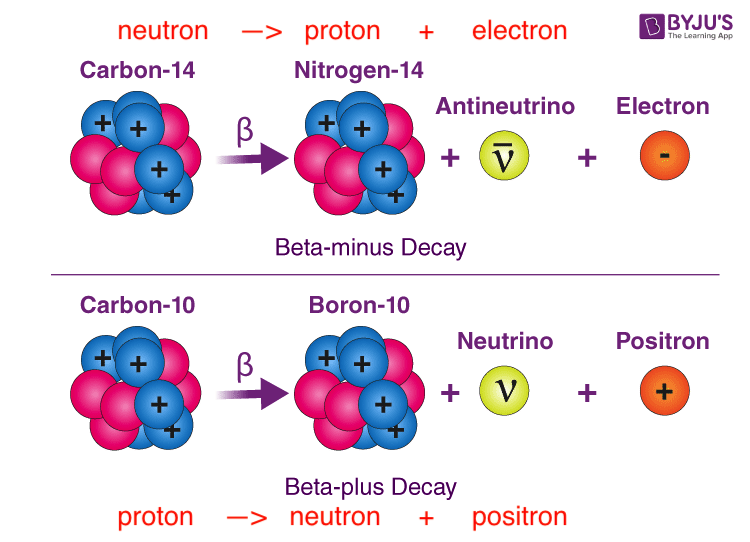
\includegraphics[width=0.9\linewidth]{beta-decay.png}
	\caption{The two types of beta decay.}
\end{wrapfigure}

During beta ($\beta^{-1}$) decay a neutron inside the nucleus changes (decays) into a proton and a high energy electron is emitted. This changing of a neutron to a proton increases the atomic number of the atom by one, and therefore changes the element!

The emitted high-energy electron can travel up \fillinunderline{to 90\% the speed of light} due to its very small mass, and has a medium range in the atmosphere (\fillinunderline{approximately 30cm}). It is able to pass through a sheet of paper but will be stopped by a more dense material e.g. 5mm of aluminium. It is said to have \fillinunderline{medium ionising ability} and can disrupt chemical bonding on impact.

Notice how there are two options for beta decay in the diagram to the right. \textbf{In both cases electric charge is conserved}.

\section{Gamma Decay}

\begin{wrapfigure}[14]{r}{0.4\linewidth}
	\centering
	% Source: https://en.wikipedia.org/wiki/Gamma_ray
	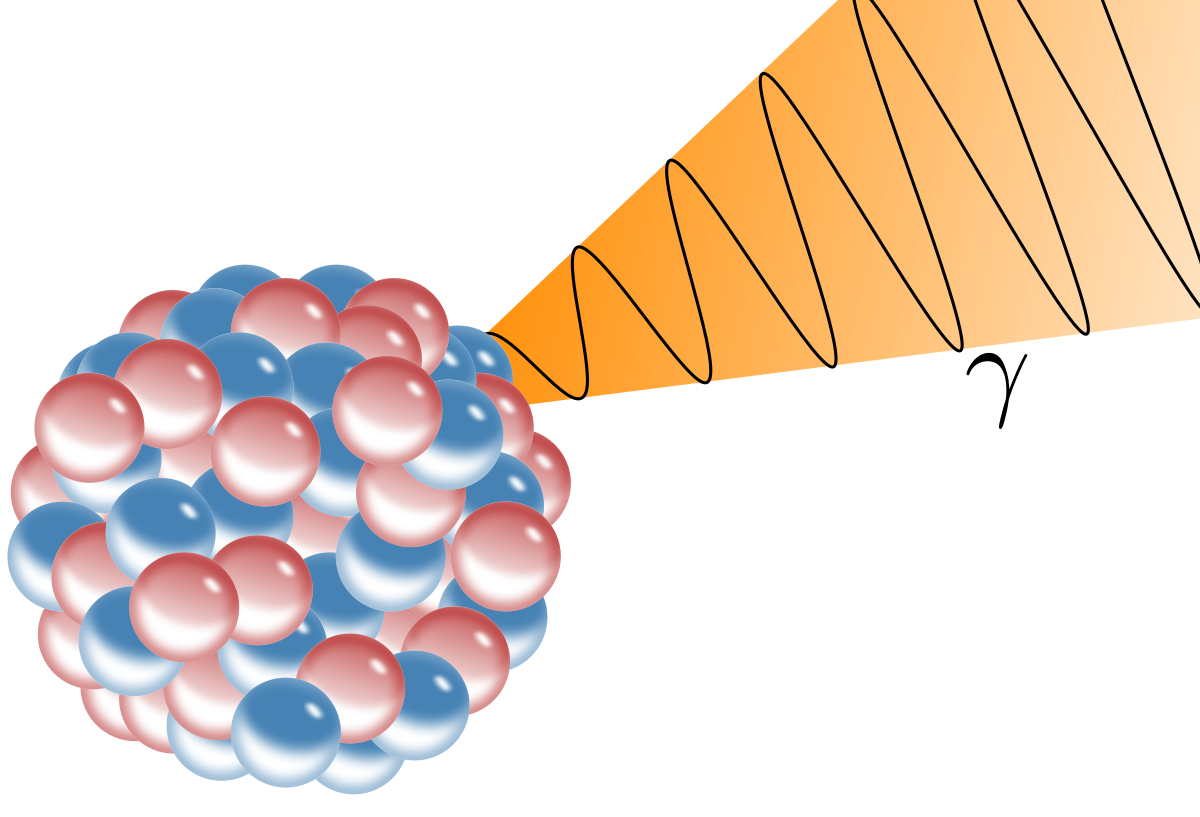
\includegraphics[width=0.9\linewidth]{gamma-decay.png}
	\caption{Notice that the nucleus stays the same.}
\end{wrapfigure}

Gamma ($\gamma$) radiation is a form of high-energy electromagnetic radiation, and is not a particle at all. It is instead an electromagnetic wave with an \fillinunderline{extremely high frequency}. This kind of radiation occurs when a nucleus is left in an \textit{excited state} after undergoing alpha or beta decay. It is a way for the nucleus to release energy.

Due to being electromagnetic radiation, it travels at \fillinunderline{the speed of light} and will travel through large volumes of atmosphere. It requires several centimetres of dense metal (e.g. lead) to block gamma radiation, and due to its lack of mass, \fillinunderline{has very little ionising ability}.

\section{Ngohe: Radiation Protection}
Draw an arrow from each type of radiation, stopping the arrow at the material that is capable of blocking it.

\begin{figure}[ht]
	\centering
	% Source: Finn Le Sueur
	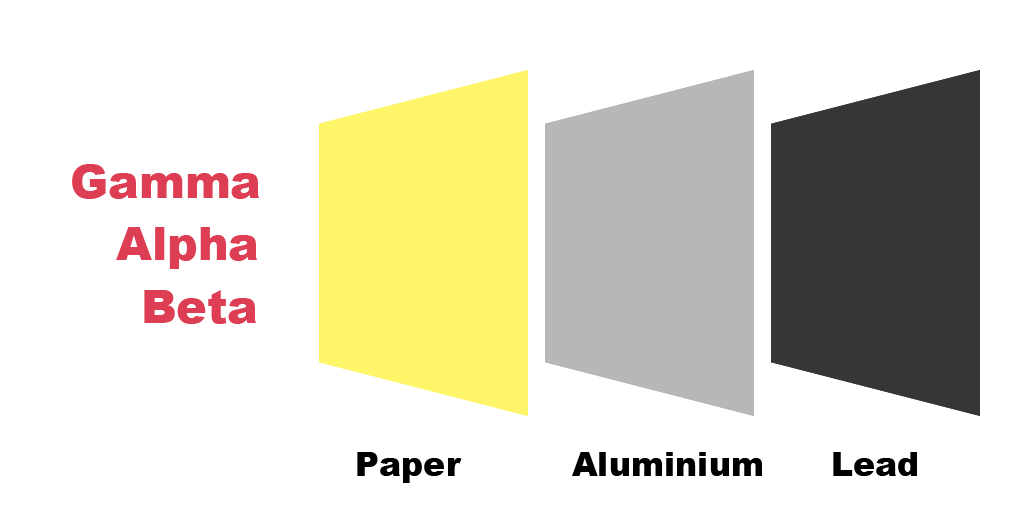
\includegraphics[width=0.9\linewidth]{radiation-penetration.png}
\end{figure}

\section{Whakawai: Types of Radiation}

\noindent{Summarise the types of radiation below.}

\begin{table}[ht]
\centering
\begin{tabular}{l|l|l|p{2cm}|l|}
\cline{2-5}
                                              		& \textbf{Mass \#} 		& \textbf{Charge} 		& \textbf{Speed} 				& \textbf{Ionising Ability} \\ \hline
\multicolumn{1}{|l|}{\textbf{Alpha Particle}} 		& \fillinblank{Large}   & \fillinblank{+2}      & \fillinblank{10\% of light}   & \fillinblank{High} 		\\ \hline
\multicolumn{1}{|l|}{\textbf{Beta Minus Particle}}  & \fillinblank{Small}   & \fillinblank{-1}      & \fillinblank{90\% of light}   & \fillinblank{Medium} 		\\ \hline
\multicolumn{1}{|l|}{\textbf{Gamma Ray}}      		& \fillinblank{None}    & \fillinblank{None}    & \fillinblank{speef of light}  & \fillinblank{Low} 		\\ \hline
\end{tabular}
\end{table}

\begin{enumerate}
	\item State which elements tend to be naturally radioactive and explain why.
	\fillinblank{Elements where the strong nuclear force that binds nucleons together is not strong enough to overcome the electromagnetic repulsive force between protons. This is 83 and up.}
	\StudentVSpace{3cm}
	
	\item Identify which of the three types of radiation is being described below.
	\begin{enumerate}
		\item It can only travel a few cm in air.\\ \fillinspace{Alpha radiation}
		\item It will pass through aluminium sheet but is stopped by a few mm of lead.\\ \fillinspace{Beta radiation}
		\item It is stopped by a sheet of paper.\\ \fillinspace{Alpha radiation}
		\item It will pass through less than a few mm of lead.\\ \fillinspace{Gamma radiation}
		\item It is highly ionising.\\ \fillinspace{Alpha radiation}
		\item It is not deflected by a magnetic field.\\ \fillinspace{Gamma radiation}
	\end{enumerate}
	\item When the three types of radiation are passed through a magnetic field they separate into three beams as shown. Identify which beam is which.
	\begin{figure}[ht]
    	\centering
    	% Source: Finn Le Sueur
    	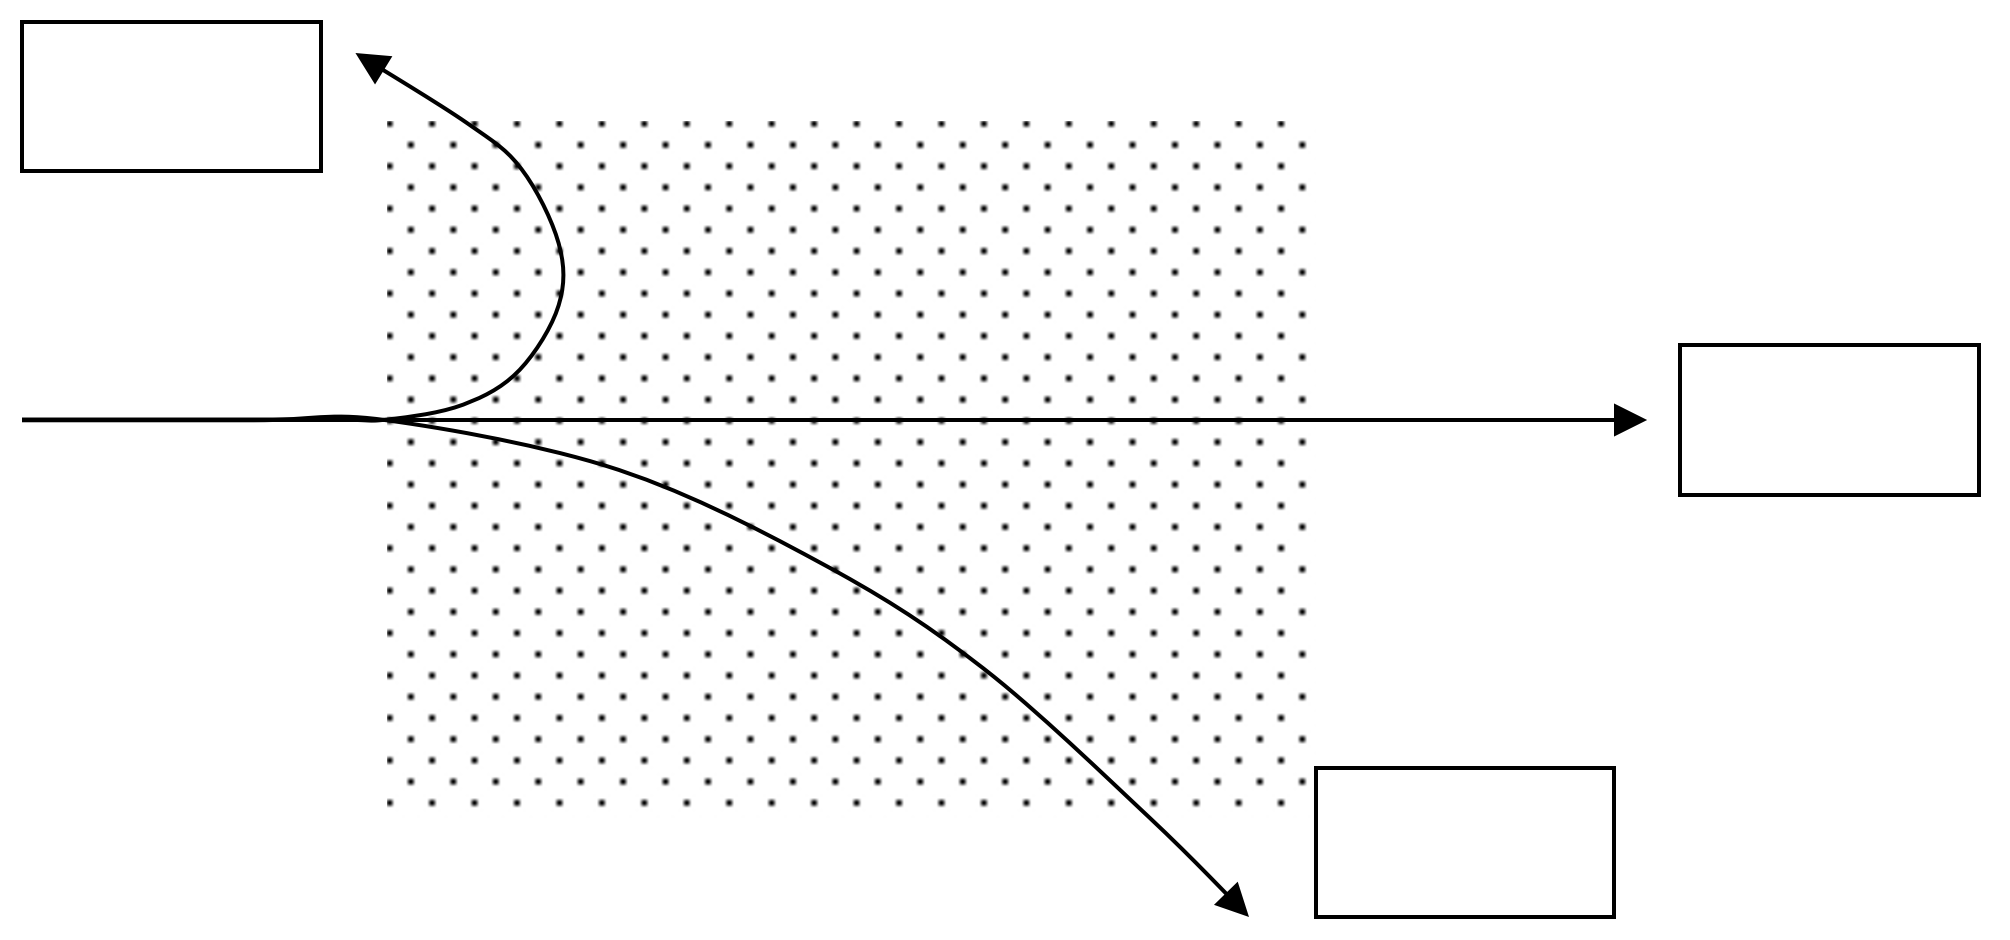
\includegraphics[width=0.8\linewidth]{radiation-magnetic-field.png}
    \end{figure}
	\item Describe what happens to the atomic number and mass number of a nucleus which emits a beta minus particle.\vspace{1.5cm}
\end{enumerate}

\newpage
\subsection{Whakamātau: Background Radiation}
All around us in the crust of Earth are a wide variety of elements. Some are even radioactive! These elements decay over time and give off a low level of radiation. Some radiation comes from interstellar space, although the majority is deflected by the Van Allen Belt.

 Thankfully we are evolved to live with this level of radiation -- our cells incorporate mechanisms to fix small mutations in our DNA. A device used to measure the amount of \textit{activity} of radiation is called a Geiger Counter. It emits a sound when it detects either alpha, beta or gamma radiation.

\begin{enumerate}
	\item Turn the geiger counter on
	\item Count the number of ticks over a period of four minutes\vspace{0.5cm}
	\item Find the \textit{activity per minute}.\vspace{0.5cm}
	\item Use paper and a sheet of metal to try and figure out the main type of radiation being detected.\vspace{1.5cm}
	\item Why do you think it is this type?\vspace{1cm}
\end{enumerate}


% =========================
%  4. Nuclear Equations
% =========================
\newpage
\chapter{Nuclear Equations}

\noindent\textbf{Learning Outcomes}
\begin{nwa}
	\item Balance nuclear equations using the knowledge of the conservation of atomic and mass numbers.
\end{nwa}

An equation for a nuclear reaction looks a lot like a regular chemical reaction. The reactants go on the left, and the products (daughter products) go on the right. We also use an arrow in the middle. The main change is that we indicate the mass an atomic numbers to the left of each atom. $M$ represents the \fillinunderline{mass number}, $A$ represents the \fillinunderline{atomic number} and $X$ represents \fillinunderline{the symbol for the atom}.

\begin{align*}
	{}^{M}_{A}X
\end{align*}

\noindent\textbf{Pātai}: In the space provided write the nuclear symbols for Thorium, Plutonium, Americium and Gold.

\vspace{1cm}

\vspace{0.25cm}\noindent State the number of protons and neutrons in the following nuclides.
\begin{enumerate}
	\item ${}^{222}_{86}Rn$: \fillinspace{86 protons, 136 neutrons}
	\item ${}^{238}_{92}U$: \fillinspace{92 protons, 146 neutrons}
	\item ${}^{63}_{29}Cu$: \fillinspace{29 protons, 34 neutrons}
	\item ${}^{27}_{13}Al$: \fillinspace{13 protons, 14 neutrons}
\end{enumerate}

\vspace{0.25cm}\noindent Write the following nuclides in their symbol form.
\begin{enumerate}
	\item A nucleus of carbon with 6 protons and 8 neutrons.\\ \fillinspace{${}^{14}_{6}C$}
	\item A nucleus of sulfur with 16 protons and 17 neutrons.\\ \fillinspace{${}^{33}_{16}S$}
	\item A nucleus of helium with 2 neutrons.\\ \fillinspace{${}^{4}_{2}He$}
	\item A nucleus of hydrogen with no neutrons.\\ \fillinspace{${}^{1}_{1}H$}
	\item A nucleus of nitrogen with a mass number of 16.\\ \fillinspace{${}^{16}_{7}N$}
	\item A nucleus of potassium with 20 neutrons.\\ \fillinspace{${}^{20}_{39}K$}
	\item A nucleus of an atom with 56 protons and 84 neutrons.\\ \fillinspace{${}^{140}_{84}Po$}
\end{enumerate}

\section{Alpha Decay}
In alpha ($\alpha$) decay a helium nucleus is emitted from the parent atom. This means that the atom loses two protons and two neutrons.
This means that the atomic number \fillinunderline{decreases} by \fillinunderline{two}, and the mass number \fillinunderline{decreases} by \fillinunderline{two}.

\noindent\textbf{Pātai}: Write the nuclear symbol for an alpha particle (two options):
\vspace{0.5cm}

\noindent\textbf{Pātai}: Use your knowledge of alpha decay to predict what atom would be produced.

\begin{table}[ht]
\centering
\begin{tabular}{|l|p{3cm}|p{3cm}|}
\hline
                            & \textbf{Before} & \textbf{After} \\ \hline
\textbf{Atom}               & Thallium-214    &                \\ \hline
\textbf{Number of Protons}  &                 &                \\ \hline
\textbf{Number of Neutrons} &                 &                \\ \hline
\textbf{Atomic Number}      &                 &                \\ \hline
\textbf{Mass Number}        &                 &                \\ \hline
\end{tabular}
\end{table}

\noindent\textbf{Pātai}: Next, we should attempt to write this decay as a nuclear equation where Thallium-214 is the reactant, and the daughter atom and alpha particle are the products.
\vspace{1cm}

\section{Beta Decay}
In beta ({$\beta^{-1}, e^{-1}$) decay a neutron turns into a proton and a \fillinunderline{high speed electron} is emitted from the nucleus. This means that the atomic number \fillinunderline{increases} by \fillinunderline{one}, and the mass number \fillinunderline{stays the same}.

\noindent\textbf{Pātai}: Write the nuclear symbol for a beta particle (two options):
\vspace{1.5cm}

\noindent\textbf{Pātai}: Use your knowledge of beta decay to predict what atom would be produced:

\begin{table}[ht]
\centering
\begin{tabular}{|l|p{3cm}|p{3cm}|}
\hline
                            & \textbf{Before} & \textbf{After} \\ \hline
\textbf{Atom}               & Polonium-218    &                \\ \hline
\textbf{Number of Protons}  &                 &                \\ \hline
\textbf{Number of Neutrons} &                 &                \\ \hline
\textbf{Atomic Number}      &                 &                \\ \hline
\textbf{Mass Number}        &                 &                \\ \hline
\end{tabular}
\end{table}

\noindent\textbf{Pātai}: Next we should attempt to write this decay as a nuclear equation where Polonium-218 is the reactant, and the daughter atom and beta particle are the products.
\vspace{1.5cm}

\section{Positron Emission}
Due to the symmetrical nature of Physics, each particle has an \textit{antiparticle}. In this case, this means that \textit{electrical charge can be conserved} if the opposite of beta decay occurs. This means that a single proton turns into a neutron and emits a positron (think: a positive electron). This means that the atomic number \fillinunderline{decreases} by \fillinunderline{one}, and the mass number \fillinunderline{stays the same}.

\noindent\textbf{Pātai}: Write the nuclear symbol for a positron (two options):
\vspace{1.5cm}

\noindent\textbf{Pātai}: An example atom that undergoes positron decay is Magnesium-23. Use your knowledge of beta decay to predict what atom would be produced:\vspace{1.5cm}

\begin{table}[ht]
\centering
\begin{tabular}{|l|p{3cm}|p{3cm}|}
\hline
                            & \textbf{Before} & \textbf{After} \\ \hline
\textbf{Atom}               & Magnesium-23    &                \\ \hline
\textbf{Number of Protons}  &                 &                \\ \hline
\textbf{Number of Neutrons} &                 &                \\ \hline
\textbf{Atomic Number}      &                 &                \\ \hline
\textbf{Mass Number}        &                 &                \\ \hline
\end{tabular}
\end{table}

\noindent\textbf{Pātai}: Next we should attempt to write this decay as a nuclear equation where Magnesium-23 is the reactant, and the daughter atom and positron are the products.
\vspace{1cm}

\section{Gamma Decay}
In gamma ($\gamma$) decay an excited nucleus emits high-energy electromagnetic waves in the form of gamma radiation. The nucleus does not emit any particles - it only becomes more \textit{relaxed}. This means that the atomic and mass numbers \fillinunderline{stay the same}.

\noindent\textbf{Pātai}: Write the nuclear symbol for a gamma ray (one option):
\vspace{0.5cm}

\noindent\textbf{Pātai}: An example of gamma decay is after Cobolt-60 has decayed to Nickel-60 via beta decay. The Nickel-60 atom is in an excited (high energy state) and needs to emit some energy. Use your knowledge of gamma decay to predict what atom would be produced:

\begin{table}[ht]
\centering
\begin{tabular}{|l|p{3cm}|p{3cm}|}
\hline
                            & \textbf{Before} & \textbf{After} \\ \hline
\textbf{Atom}               & Nickel-60       &                \\ \hline
\textbf{Number of Protons}  &                 &                \\ \hline
\textbf{Number of Neutrons} &                 &                \\ \hline
\textbf{Atomic Number}      &                 &                \\ \hline
\textbf{Mass Number}        &                 &                \\ \hline
\end{tabular}
\end{table}

\noindent\textbf{Pātai}: Next we should attempt to write this decay as a nuclear equation where Nickel-60 is the reactant, and the daughter atom and gamma ray are the products.
\vspace{1.5cm}

\section{Whakawai: Decay Equations}
\textbf{Write the nuclear equations for these reactions}. For double decays, write two equations and then combine them into a single equation.
\begin{enumerate}[itemsep=2cm]
	\item An alpha decay of Polonium-218
	\item A beta decay of Hydrogen-3
	\item A gamma decay of Carbon-14
	\item An absorption of a neutron by Carbon-13 ($C-13 + n$)
	\item A double alpha decay of Uranium-234\vspace{1cm}
	\item A double beta decay of Thorium-234\vspace{1cm}
\end{enumerate}

\newpage
\section{Whakawai: Types of Radiation}
Complete the two nuclear equations below with appropriate symbols and numbers to identify the type of radiation emitted. 

\begin{enumerate}[itemsep=1cm]
	\item ${}^{90}_{38}Sr \rightarrow {}^{90}_{39}Y + ...$ \hspace{2cm} Name of Radiation:
	\item ${}^{60}_{27}Co \rightarrow {}^{60}_{27}Co + ...$ \hspace{2cm} Name of Radiation:
	\item Uranium-238 decays to thorium (Th) by emitting an alpha particle. Complete the equation for this reaction using appropriate symbols and numbers.\\\\
	${}^{238}_{92}U \rightarrow$
	\item What is meant by the term \textit{ionising}?
	\item Which type of radiation is most strongly ionising?
	\item An electron can be emitted from a radioactive nucleus even though it cannot exist inside the nucleus. Where does that electron come from?\vspace{1cm}
	\item As part of an experiment, Rutherford placed an alpha particle emitter into a jar. When the jar was later tested it contained the gas helium that was not previously present. Explain how the helium was formed.\vspace{1cm}
	\item The isotope Radon-222 (${}^{222}_{86}Rn$) undergoes two consecutive radioactive decays and turns into the isotope Polonium-218 (${}^{218}_{84}Po$). Write equations to determine the TWO separate emissions. Name the emissions.\vspace{1cm}
\end{enumerate}

\subsection{Pātai: Radiation in a Magnetic Field}
Radioactivity can occur in three distinct forms. The following diagram shows a radioactive source whose emission comprises all three forms. The three emission forms are being separated as they pass through a uniform magnetic field directed into the page, as indicated by the crosses.

\begin{figure}[ht]
	\centering
	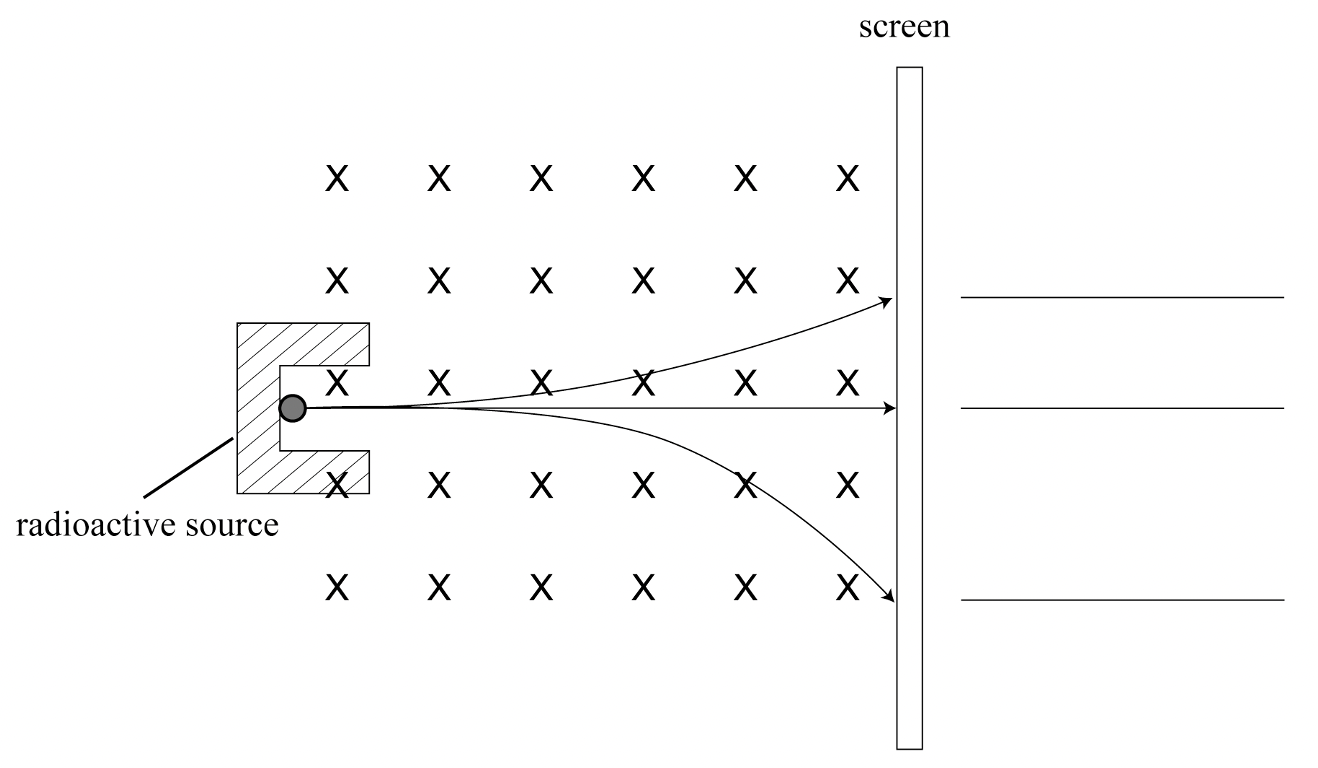
\includegraphics[width=0.8\linewidth]{radiation-magnetic-field-2.png}
\end{figure}

\begin{enumerate}
	\item Name each emission form on the appropriate line to the right of the screen.
	\item Explain the path of the top particle by explaining the relevant RH rule and relate the amount of deflection to the force experienced ($F=Bqv$) and the properties of the particle.\vspace{3cm}
	\item Explain the path of the middle particle by explaining the relevant RH rule and relate the amount of deflection to the force experienced ($F=Bqv$) and the properties of the particle.\vspace{3cm}
	\item Explain the path of the bottom particle by explaining the relevant RH rule and relate the amount of deflection to the force experienced ($F=Bqv$) and the properties of the particle.\vspace{3cm}
\end{enumerate}

\newpage
\subsection{Pātai: Geiger Counter Investigation}
A student wanted to identify the type of radiation emitted from three unknown radioactive sources. She had a piece of paper, a strong magnet and a Geiger counter. The radioactive sources were attached to discs coloured red, blue and green. In the investigations, she placed each radioactive source in the position shown, and measured the radiation received by the Geiger counter.

\begin{figure}[ht]
	\centering
	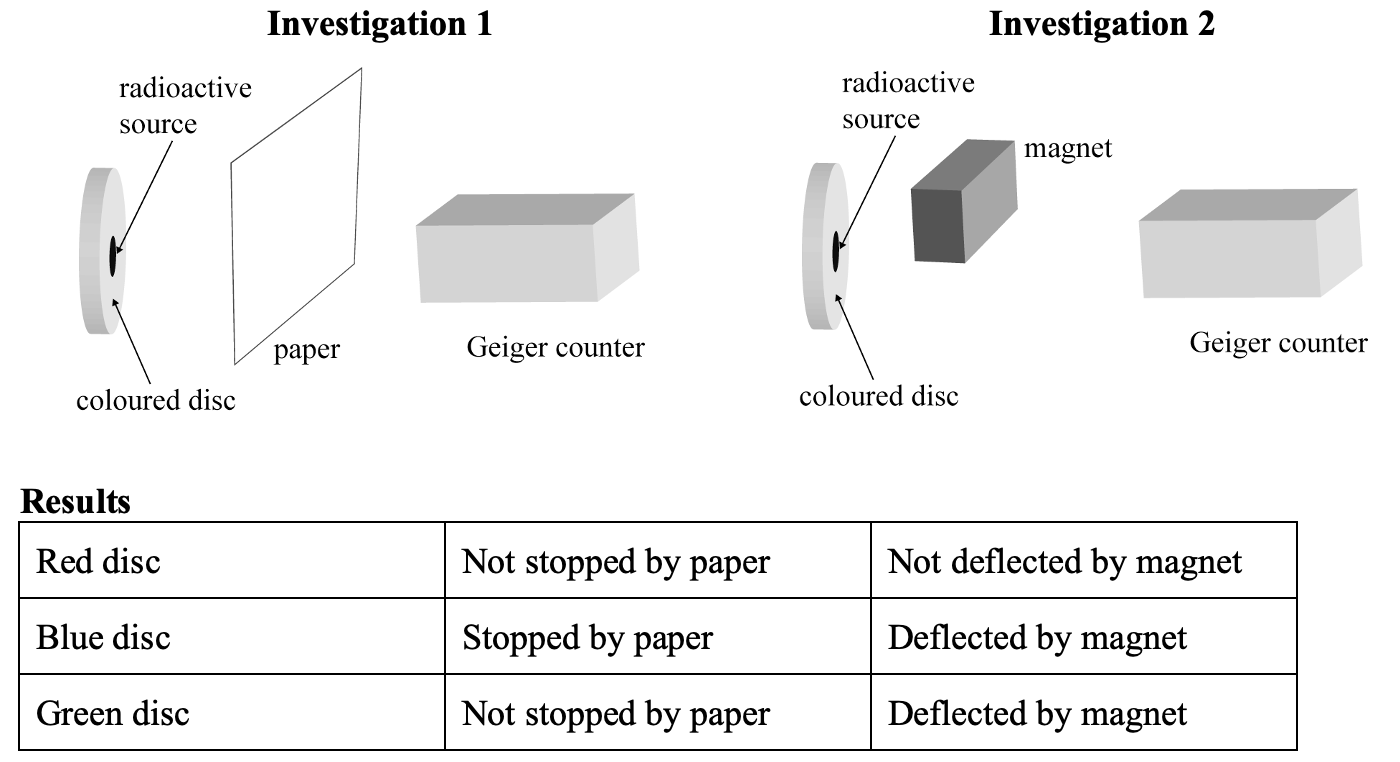
\includegraphics[width=0.8\linewidth]{geiger-investigation.png}
\end{figure}

Deduce the type of radiation emitted from each radioactive source, giving a brief explanation in each case.

\begin{enumerate}
	\item Radioactive source on red disc emits: \\
	\textbf{Explanation:}\vspace{1.5cm}
	\item Radioactive source on blue disc emits: \\
	\textbf{Explanation:}\vspace{1.5cm}
	\item Radioactive source on green disc emits: \\
	\textbf{Explanation:}\vspace{1.5cm}
\end{enumerate}

\newpage
\subsection{Pātai: Platinum}
Platinum-195 (${}^{195}_{78}Pt$) and platinum-192 (${}^{192}_{78}Pt$) are both isotopes of the same element.

\begin{enumerate}
	\item State the difference between the nuclei of platinum-192 and platinum-195.\vspace{1.5cm}
	\item What do the numbers 78 and 195 represent in the symbol?\vspace{1.5cm}
	\item Write an equation for the decay of iridium-192 to platinum and name the particle emitted.\vspace{1.5cm}
	\item What Physics principles did you use to write the above nuclear equation?\vspace{1.5cm}
	\item Technetium-99 is sometimes injected into hospital patients. Technetium-99 decays by emitting gamma rays and low energy electrons. Technetium-99 has a half life of 6 hours. Give TWO reasons why is it important for doctors to use a radioactive isotope that has a half-life of a few hours in patients.\vspace{1.5cm}
	\item Explain why it is safer to inject radioisotopes that emit gamma rays rather than those that emit alpha particles.\vspace{1.5cm}
	\item Describe and explain the changes which occur in the nucleus of a radioactive isotope, including changes of its atomic number and mass number when it decays by emitting:
	\begin{enumerate}
		\item An alpha particle\vspace{1.5cm}
		\item A beta particle\vspace{1.5cm}
	\end{enumerate}
\end{enumerate}

\subsection{Pātai: Classroom Sources}
Here we have three radioactive sources: Polonium-210 (alpha), Strontium-90 (beta) and Cobalt-60 (gamma). When the Geiger counter emits a "beep", a single nucleus has transformed via radioactive decay.
\begin{enumerate}[itemsep=1.5cm]
	\item Describe why (if) the Polonium-210 source can be detected using a Geiger counter.
	\item Write a nuclear equation describing the decay of a Polonium-210 nucleus.
	\item Describe why (if) the Strontium-90 source can be detected using a Geiger counter.
	\item Write a nuclear equation describing the decay of a Strontium-90 nucleus.
	\item Describe why (if) the Cobalt-60 source can be detected using a Geiger counter.
	\item Write a nuclear equation describing the decay of a Cobalt-60 nucleus.
\end{enumerate}


% =========================
%  5. Half-Life
% =========================
\newpage
\chapter{Half-Life}

\noindent\textbf{Learning Outcomes}
\begin{nwa}
	\item Be able to make half-life graphs
	\item Be able to interpret half-life graphs
\end{nwa}

\noindent\href{https://www.youtube.com/watch?v=zXw2cOSBB8E}{Introductory Video: https://www.youtube.com/watch?v=zXw2cOSBB8E}

\section{Whakamātau: Dice}
\begin{enumerate}
	\item In pairs, collect a container of dice from the front.
	\item Count and record the total number of dice.
	\item Roll all the dice in one go. Discard aside the dice with dots facing up, count the dice without dots and record that value (number of dice remaining).
	\item Roll all the dice in one go that did did not land with dots facing up. Discard those with dots facing up, count, record and repeat until no dice remain.
	\item Create a line graph showing the number of dice rolled (y-axis) vs the roll number (x-axis).
	\item Interpret your graph to find out how many rolls it took for your original number of dice to halve. Confirm this by checking subsequent halvings.
\end{enumerate}

\vspace{10cm}

\begin{wrapfigure}[11]{r}{0.4\linewidth}
	\centering
	\vspace{-1cm}
	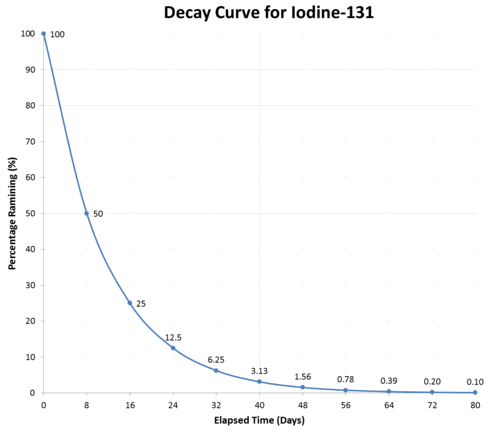
\includegraphics[width=0.9\linewidth]{iodine-131.png}
\end{wrapfigure}

What you have hopefully discovered is an exponential decay curve! This type of curve can be observed in a multitude of places in nature, but in Nuclear Physics it shows the half-life of a particular radioactive atom.

It is important to note that \textit{for any section of a decay curve, it is steeper on the left and more gentle on the right}. This means that the mass/number of atoms is changing more rapidly on the left.

\section{What is Half-Life?}

\noindent\textbf{Definition}: The time taken for half of a radioactive sample to undergo decay (half the nuclei to transform into their daughter-type)

Many things in the universe are deterministic - calculations can be performed to make accurate and specific predictions, however we are unable to predict when \textit{exactly} a particular radioactive nuclei will decay. It turns out that decay is \textit{probabilistic} and it is impossible to make a prediction for a single nuclei.

It is, however, possible to make predictions about groups of atoms using statistics (exponential decay curves).

We should also note that each different radioactive nuclei has a different half-life. Tellurium-128 is believed to have a half-life of over 128 trillion years, while Hydrogen-7 has a half-life of $23\times10^{-24}s$.


\noindent\textbf{Pātai}: If there were initially 1200 particles in a sample, fill out the number of particles left \textit{after} each half life has elapsed.

\begin{table}[h]
\centering
\begin{tabular}{c|c|c|c|}
\cline{2-4}
\textbf{}                                         & \multicolumn{3}{c|}{\textbf{Remaining}}                      \\ \hline
\multicolumn{1}{|c|}{\textbf{Half-Lives Elapsed}} & \textbf{Fraction} & \textbf{Percentage} & \textbf{Particles} \\ \hline
\multicolumn{1}{|c|}{\textbf{1}}                  &                &                   &                    \\ \hline
\multicolumn{1}{|c|}{\textbf{2}}                  &                &                   &                    \\ \hline
\multicolumn{1}{|c|}{\textbf{3}}                  &                &                 &                    \\ \hline
\multicolumn{1}{|c|}{\textbf{4}}                  &               &                 &                    \\ \hline
\multicolumn{1}{|c|}{\textbf{5}}                  &               &                &                    \\ \hline
\multicolumn{1}{|c|}{\textbf{6}}                  &               &               &                    \\ \hline
\multicolumn{1}{|c|}{\textbf{7}}                  &              &              &                    \\ \hline
\end{tabular}
\end{table}

\section{Half-Life Calculations}
Those of who are confident with their math skills will have noticed that you can formulate an equation to help you make precise predictions about the number of particles left for any given time. In Year 12 Physics we do not use a formula, rather we make more approximate predictions by creating and reading graphs. Equation use is something you may see in Year 13 and into tertiary education.
We can also perform predictions simply by \textit{dividing by two} (as above) and using this to help us make estimates.

\subsection{Method 1: Dividing}
This method is slightly less accurate in some cases than the graphical method. The half-life of Hydrogen-3 (Tritium) is approximately 12.25 years. If you found a small sample of Tritium containing 5,000,000 un-decayed nuclei.

\begin{enumerate}[itemsep=1cm]
	\item How many nuclei will be left after 12.25 years?
	\item How many nuclei will be left after 24.5 years?
	\item How many nuclei will be left after 49 years?
	\item How many nuclei will be left after 196 years?
	\item How long until there is less than 2500 un-decayed nuclei left?\vspace{1cm}
\end{enumerate}

\subsection{Method 2: Graphs}
This method can help us gain a better view when we want to know about non-integer half-lives e.g. the number of particles after 4.5 half-lives.

\noindent\textbf{Pātai}: You found a $50g$ sample of Cobalt-60 which has a half-life of 5 years.

\begin{enumerate}
    \item Sketch a mass vs. time graph of the Cobalt-60 sample over a 30-year period. Use the graph to answer the following questions:\vspace{10cm}
	\item How long it would take for the mass of the $50g$ sample to fall just below $1.17g$.\vspace{1cm}
	\item Estimate the mass of Cobalt-60 left after 12.5 years.\vspace{1cm}
	\item Estimate the number of Cobalt-60 particles after 20 years.\vspace{1cm}
\end{enumerate}

\subsection{Whakawai: Iodine-131}
Predict the amount of time until there is 37.5\% of the original sample of Iodine-131 left.

\begin{figure}[h]
	\centering
	% Source: https://chem.libretexts.org/Bookshelves/Introductory_Chemistry/The_Basics_of_GOB_Chemistry_(Ball_et_al.)/11%3A_Nuclear_Chemistry/11.02%3A_Half-Life
	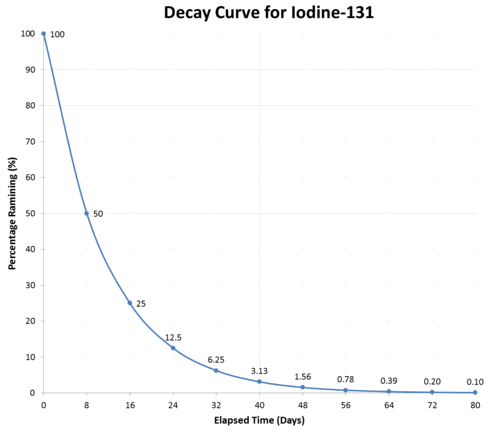
\includegraphics[width=0.75\linewidth]{iodine-131.png}
\end{figure}

\newpage
\subsection{Whakawai: Carbon-Dating}
Radio-carbon dating is used to estimate the age of objects that were once living. All living things contain a small amount of radioactive Carbon-14 (${}^{14}_{6}C$). Radioactive C-14 is created through the impact of cosimic rays with carbon in the atmosphere. This carbon is then used by plants in photosynthesis, and these plants eaten by animals.

Organisms have a relatively constant ratio of C-14 in them over their lifetime due to them continually consuming it through food. Once they die they are no long acquiring C-14 and it starts to decay away.

Carbon-14, which has a half-life of 5700 years, decays to Carbon-12. By measuring the activity of a sample of dead tissue, its approximate age can be determined. Activity is measured in counts per minute ($\frac{counts}{min}$ or $\frac{decays}{minute}$).

\begin{enumerate}[itemsep=1.5cm]
	\item Calculate the number of neutrons present in a carbon 14 nucleus.
	\item State what is meant by the term \textit{half-life}.
	\item A sample of living wood has an activity of $16counts/min$ per gram. Calculate the activity of a $20g$ sample of living wood.
	\item Hence calculate the activity of a $20g$ sample of wood from a tree that died 17,100 years ago. State the correct unit for your answer.\vspace{2cm}
	\item A $5.0g$ sample of wood from an archaeological site has an activity of $20counts/min$. Calculate the activity of the sample when the wood was living, and hence calculate how long ago the tree died.\vspace{2cm}
\end{enumerate}

\newpage
\subsection{Whakawai: Cobalt-60}
Cobalt 60 is a beta emitter used in medicine. It is created in a nuclear reactor, and decays with a half-life of 5.2 years. It is stored in a lead container until it is used.

\begin{enumerate}
	\item State why the container is made of lead.\vspace{1.5cm}
	\item In 2001, the contents of a sealed lead container were 2.0 g of radioactive Cobalt 60. Determine the approximate mass of the contents five years later. Explain your answer.\vspace{3cm}
	\item In what year will the rate of decay of the Cobalt 60 be one-quarter of what it was in 2001? \vspace{2cm}
\end{enumerate}

\newpage
\subsection{Whakawai: Iodine-131}
A sample of pure iodine-131 has a decay rate of $600s^{-1}$ (counts per second). 16 days later the decay rate has dropped to $150s^{-1}$.  Use a graph to determine the decay rate after 28 days. You must show your working.

\begin{figure}[h]
	\centering
	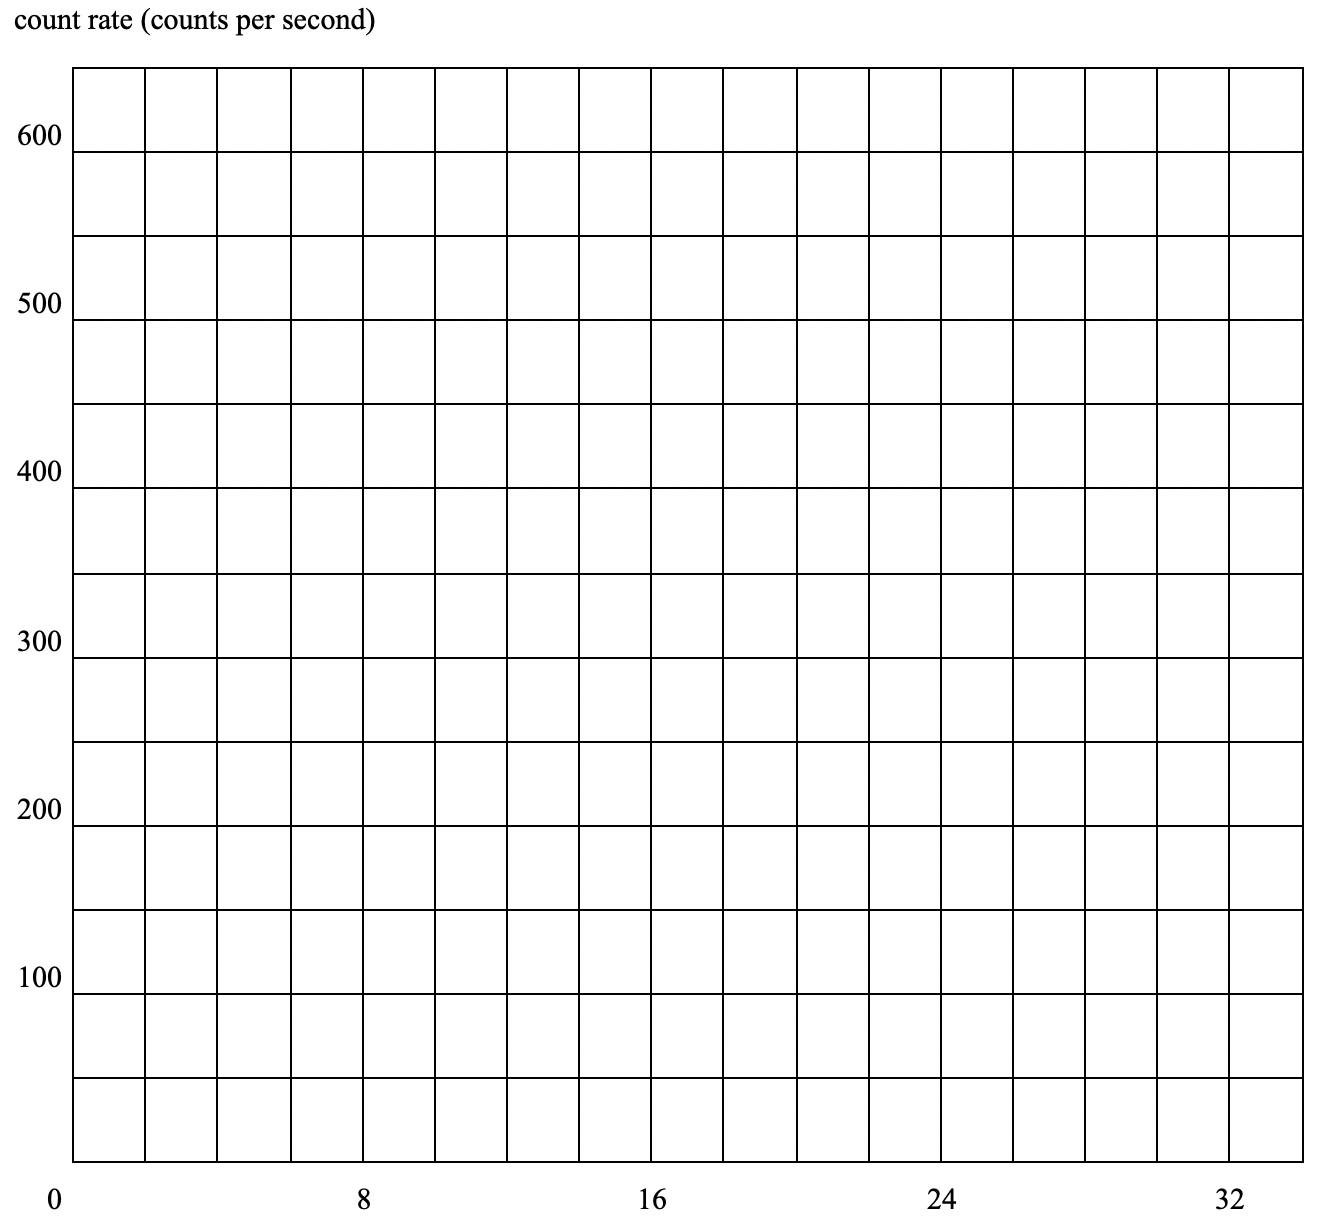
\includegraphics[width=\linewidth]{iodine-131-graph.png}
\end{figure}


% =========================
%  6. Fission and Fusion
% =========================
\newpage
\chapter{Fission and Fusion}

\noindent\textbf{Learning Outcomes}
\begin{nwa}
	\item Understand the difference between nuclear fission and fusion
	\item Use $E=mc^{2}$
	\item Use $P=\frac{E}{t}$
\end{nwa}

\noindent\href{https://www.youtube.com/watch?v=rcOFV4y5z8c}{Introductory Video: https://www.youtube.com/watch?v=rcOFV4y5z8c}

\section{Nuclear Fission}
Recall from earlier that nuclei are generally stable because the \fillinunderline{strong nuclear force} is greater than the \fillinunderline{electrostatic force}. This means that even though the protons repel each other, the nucleus does not break apart. Also recall that atoms with a nucleus that is too large in volume can be unstable (radioactive). This is because the electrostatic force is greater than the strong nuclear force, and the atom can then break down (decay) via alpha or beta/position emission.

\begin{figure}[h]
	\centering
	% Source: https://ebrary.net/55394/sociology/neutron_capture_processes_heaviest_elements
	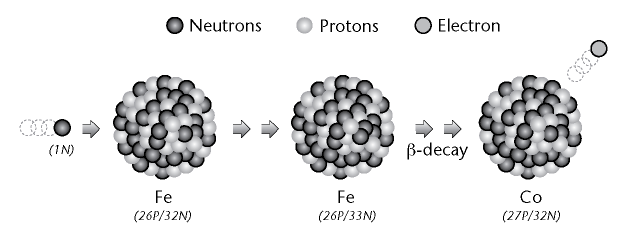
\includegraphics[width=0.7\linewidth]{neutron-bombardment.png}
\end{figure}

By colliding high-speed neutrons with an already large nucleus, the neutron can sometimes be incorporated into the nucleus via the \fillinunderline{strong nuclear force}. This in turn causes the electrostatic force to now become larger than the strong nuclear force and \textbf{the nuclei to break apart in nuclear fission}. This is the process through which nuclear reactors produce energy here on Earth.

\subsection{Pātai: Fission of Uranium}
Uranium-235 is bombarded with a high speed neutron. The resulting nucleus becomes radioactive and decays into two daughter nuclei: Krypton-92 and Barium-141.

\begin{enumerate}[itemsep=1.5cm]
	\item Write a nuclear equation describing the bombardment and fission of U-235
	\item What is the third product? How did you determine it - what was conserved?\vspace{2cm}
\end{enumerate}

\section{Nuclear Fusion}

\begin{wrapfigure}[15]{r}{0.4\linewidth}
	\centering
	% Source: https://en.wikipedia.org/wiki/Nuclear_fusion
	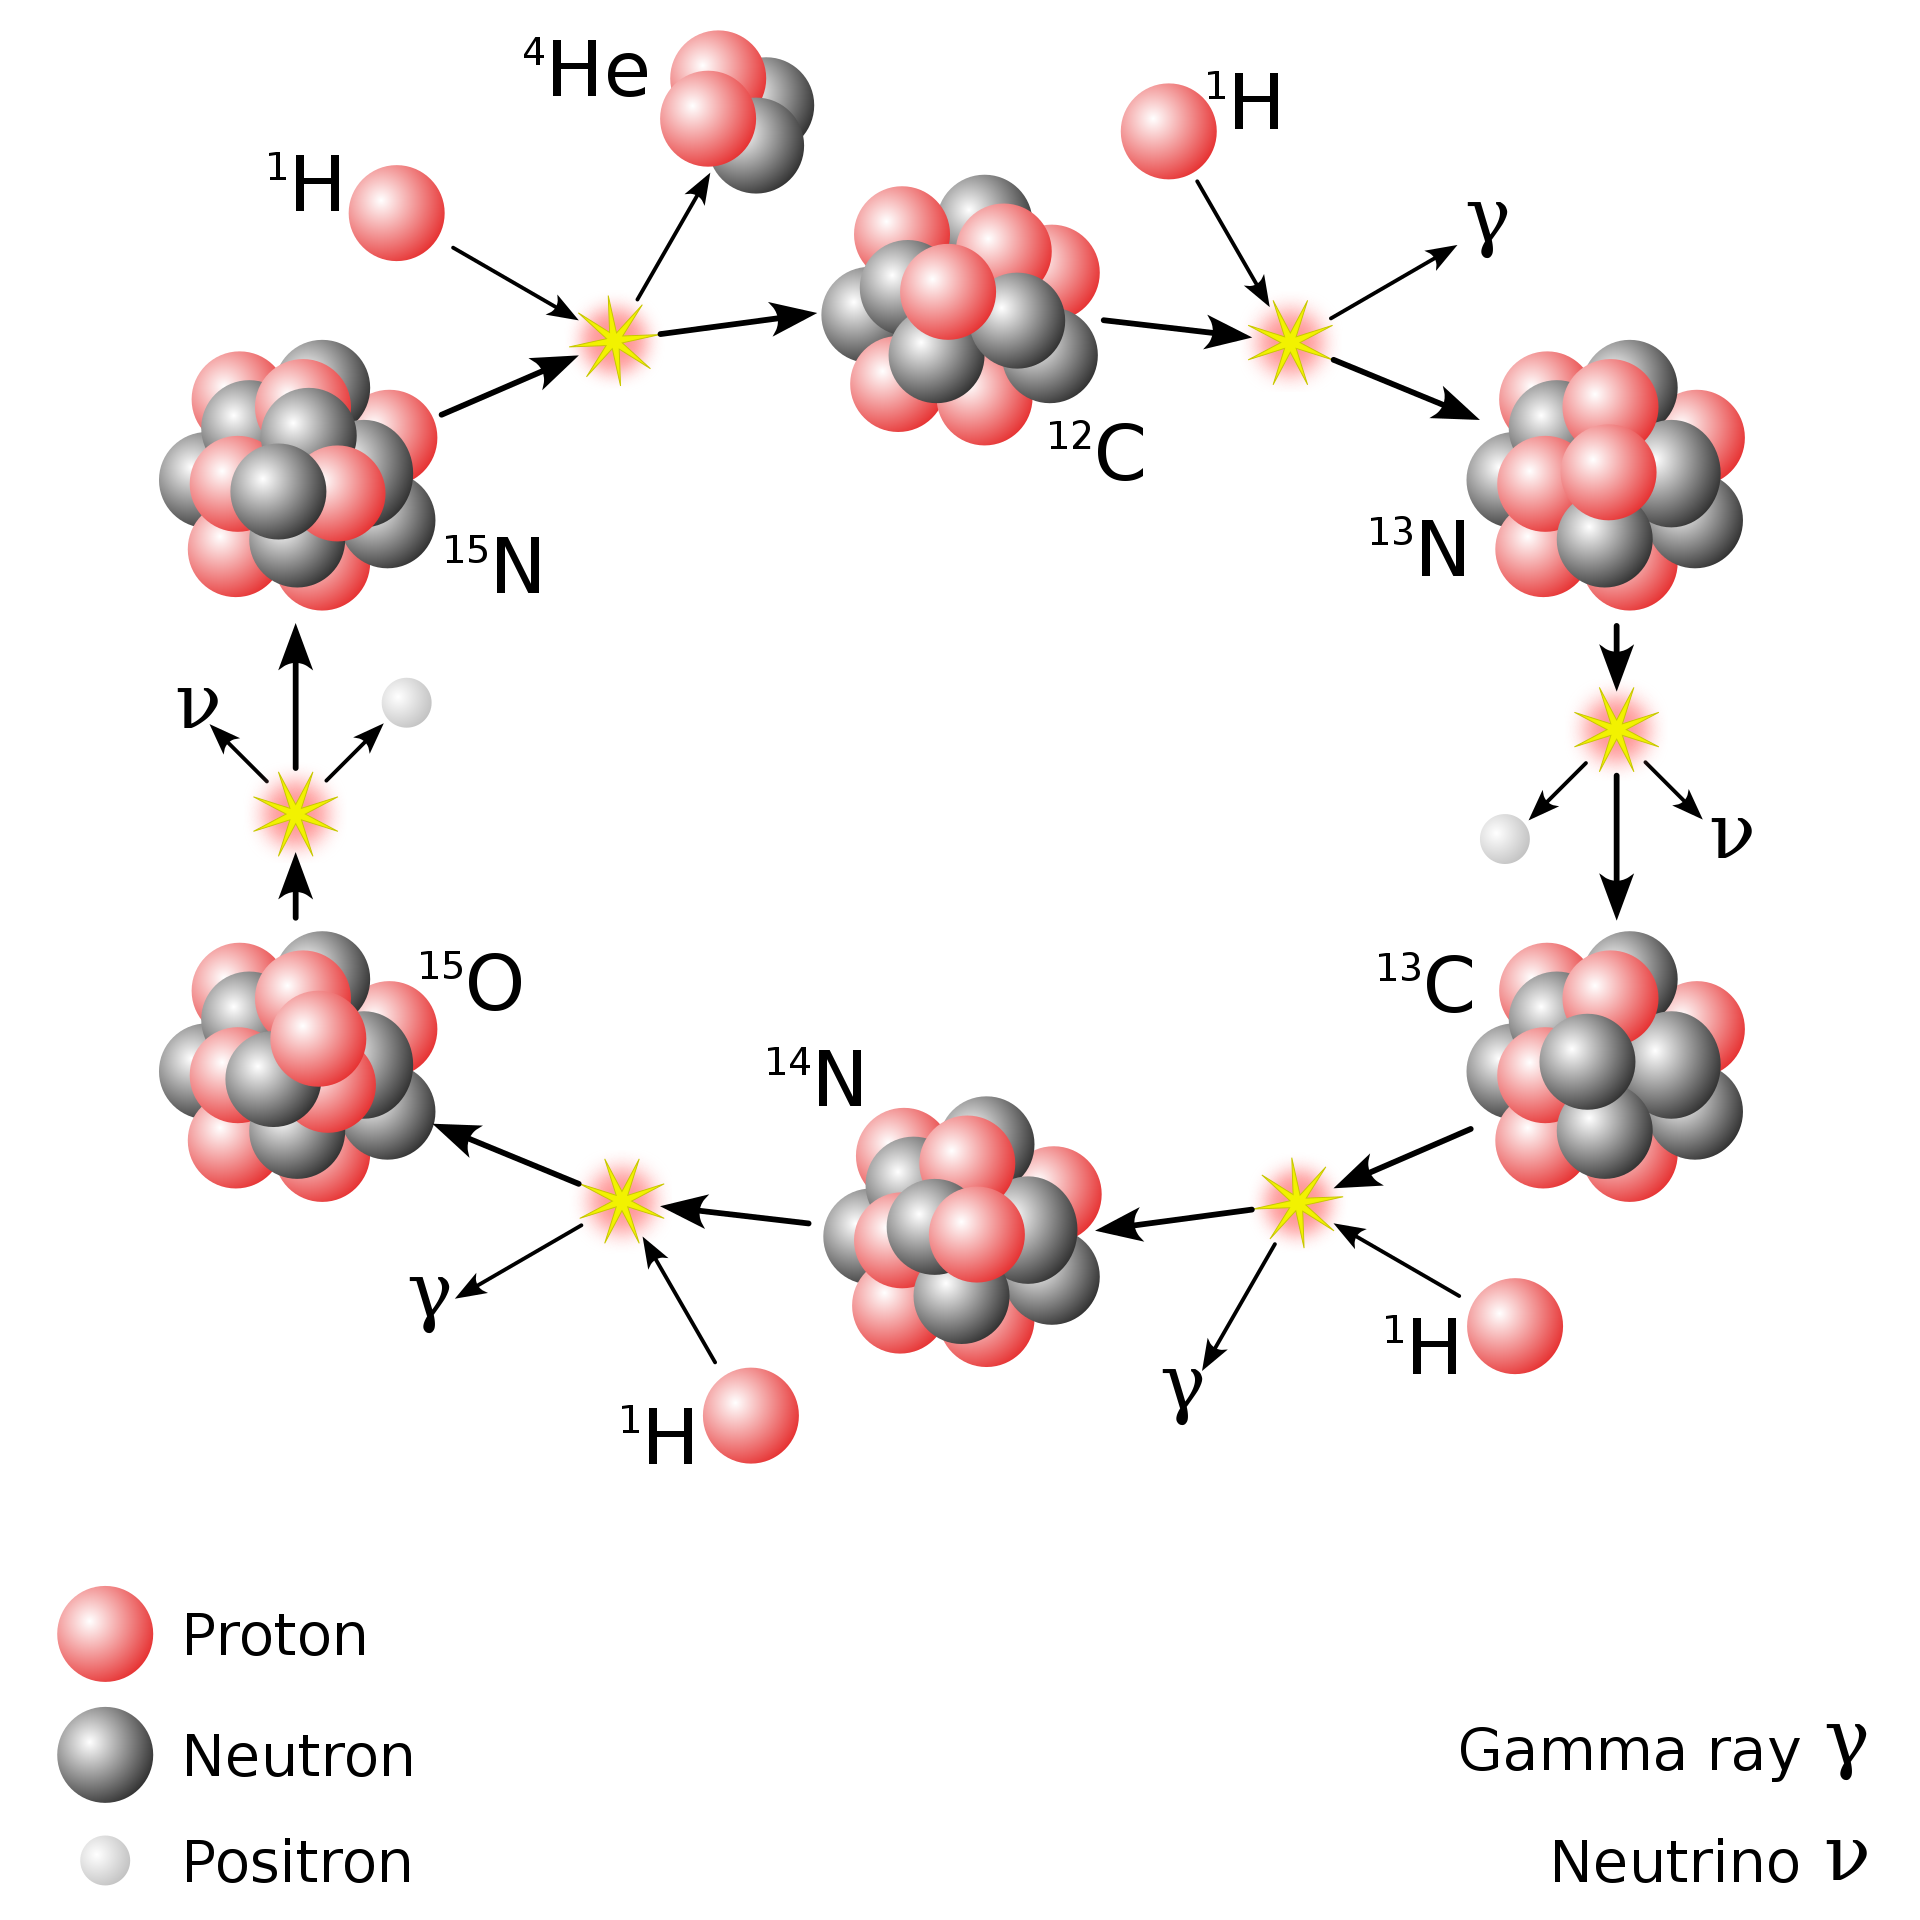
\includegraphics[width=0.9\linewidth]{CNO-cycle.png}
\end{wrapfigure}

Unlike Nuclear Fission, with fusion we can add whole nuclei together! This is the process through which stars produce energy. Fusion typically requires very high temperatures and pressures in order to get the nuclei close enough to combine. It is for this reason that we struggle to create self-sustaining fusion reactions here on Earth - it is hard to create and maintain these conditions.

However, it is important to note that fusing nuclei smaller than iron produces energy, while trying to fuse nuclei larger than iron requires more energy than is produced. We will see this concept again later!

\subsection{Pātai: Fusion of Hydrogen}
In the Sun deuterium (H-2) and tritium (H-3) are fused together to create helium (He-4) and one other product.

\begin{enumerate}[itemsep=1.5cm]
	\item Write a nuclear equation describing the fusion of H-2 and H-3
	\item What is the second product? How did you determine it - what was conserved?\vspace{2cm}
\end{enumerate}

\section{Mass-Energy Equivalence}
You probably know Einstein's most famous formula were $E$ is energy, $m$ is mass and $c$ is the speed of light:

\begin{align*}
	E=mc^{2}
\end{align*}

Because the speed of light is so large, this implies that a small amount of mass can be converted into a large amount of energy.

\subsection{Pātai: Antimatter}
Let's pretend $2g$ of material is converted directly into energy (this would be a matter-antimatter collision). Calculate the amount of energy generated by this reaction, given $c\approx3\times10^{8}ms^{-1}$.
\kufss

\noindent\href{https://www.youtube.com/watch?v=HEYbgyL5n1g}{Introductory Video: https://www.youtube.com/watch?v=HEYbgyL5n1g}

\section{How Fission and Fusion Produce Energy}
It turns out that if you measure the mass of the reactants and products of a nuclear reaction, mass is not (exactly) conserved. Instead, the products have slightly less total mass than the reactants. This means that some mass was lost. Where did it go? It turned into energy via mass-energy equivalence.

\subsection{Pātai: Fusion of Deuterium}
\noindent\href{https://www.youtube.com/watch?v=mZsaaturR6E}{Introductory Video: https://www.youtube.com/watch?v=mZsaaturR6E}
\begin{align*}
    & {}^{3}_{1}H + {}^{2}_{1}H \rightarrow {}^{4}_{2}He + {}^{1}_{0}n
\end{align*}

\begin{itemize}
	\item Tritium (${}^{3}_{1}H$) $= 5.00641 \times 10^{-27} kg$
	\item Deuterium (${}^{2}_{1}H$) $= 3.3436 \times 10^{-27} kg$
	\item Helium (${}^{4}_{2}He$) $= 6.64466 \times 10^{-27} kg$
	\item Neutron (${}^{1}_{0}n$) $= 1.67493 \times 10^{-27} kg$
\end{itemize}

\noindent Use these data to answer the following questions.

\begin{enumerate}[itemsep=2cm]
	\item Calculate the total mass of the reactants.
	\item Calculate the total mass of the products.
	\item Calculate the amount of mass lost during the reaction.
	\item Calculate the energy produced during this reaction.
	\item Calculate the power output of this reaction if it took $0.0001s$ to occur ($P=\frac{E}{t}$).\vspace{2cm}
\end{enumerate}

\subsection{Pātai: Fission of U-235}
A nuclear power plant in the US can produce $1GW$ of power through neutron bombardment of U-235 and consequently, its fission. This fission produces Ba-141, Kr-92 and three neutrons.

\begin{itemize}
	\item $U-235 = 390.2480 \times 10^{-27} kg$
	\item $Ba-141 = 233.9616 \times 10^{-27} kg$
	\item $Kr-92 = 152.5794 \times 10^{-27} kg$
	\item $Neutron = 1.67493 \times 10^{-27} kg$
\end{itemize}

\noindent Use these data to answer the following questions.
\begin{enumerate}[itemsep=2cm]
	\item Write an equation describing this nuclear reaction.
	\item Calculate the total mass of the reactants.
	\item Calculate the total mass of the products.
	\item Calculate the amount of mass lost during the reaction.
	\item Calculate the energy produced during this reaction.
	\item If the plant is running for one year, calculate the mass of U-235 required. Start by calculating the amount of mass needed to produce $1GW$ of power, and then scale that up to the length of one year.\vspace{4cm}
\end{enumerate}

\subsection{Pātai: Smoke Alarm}
One particular type of smoke detector used in homes contains a radioactive material called americium. When a nucleus of americium decays it emits an alpha particle. The emitted alpha particles ionise the air inside the smoke detector. These ions travel between positive and negative plates inside the detector - thus creating a current and completing the circuit! This is what causes the alarm to sound.

\begin{align*}
	{}^{241}_{95}Am \rightarrow {}^{4}_{2}He + {}^{237}_{93}Np + energy
\end{align*}

\begin{itemize}
	\item Helium $= 6.64476 \times 10^{-27}kg$
	\item Neptunium $= 393.54874 \times 10^{-27}kg$
	\item Americium $= 400.20350 \times 10^{-27}kg$
\end{itemize}

Given the above data, calculate the quantity of energy released in the alpha decay of a nucleus of americium.\vspace{4cm}

\newpage
% \addcontentsline{toc}{chapter}{Periodic Table of Elements} 
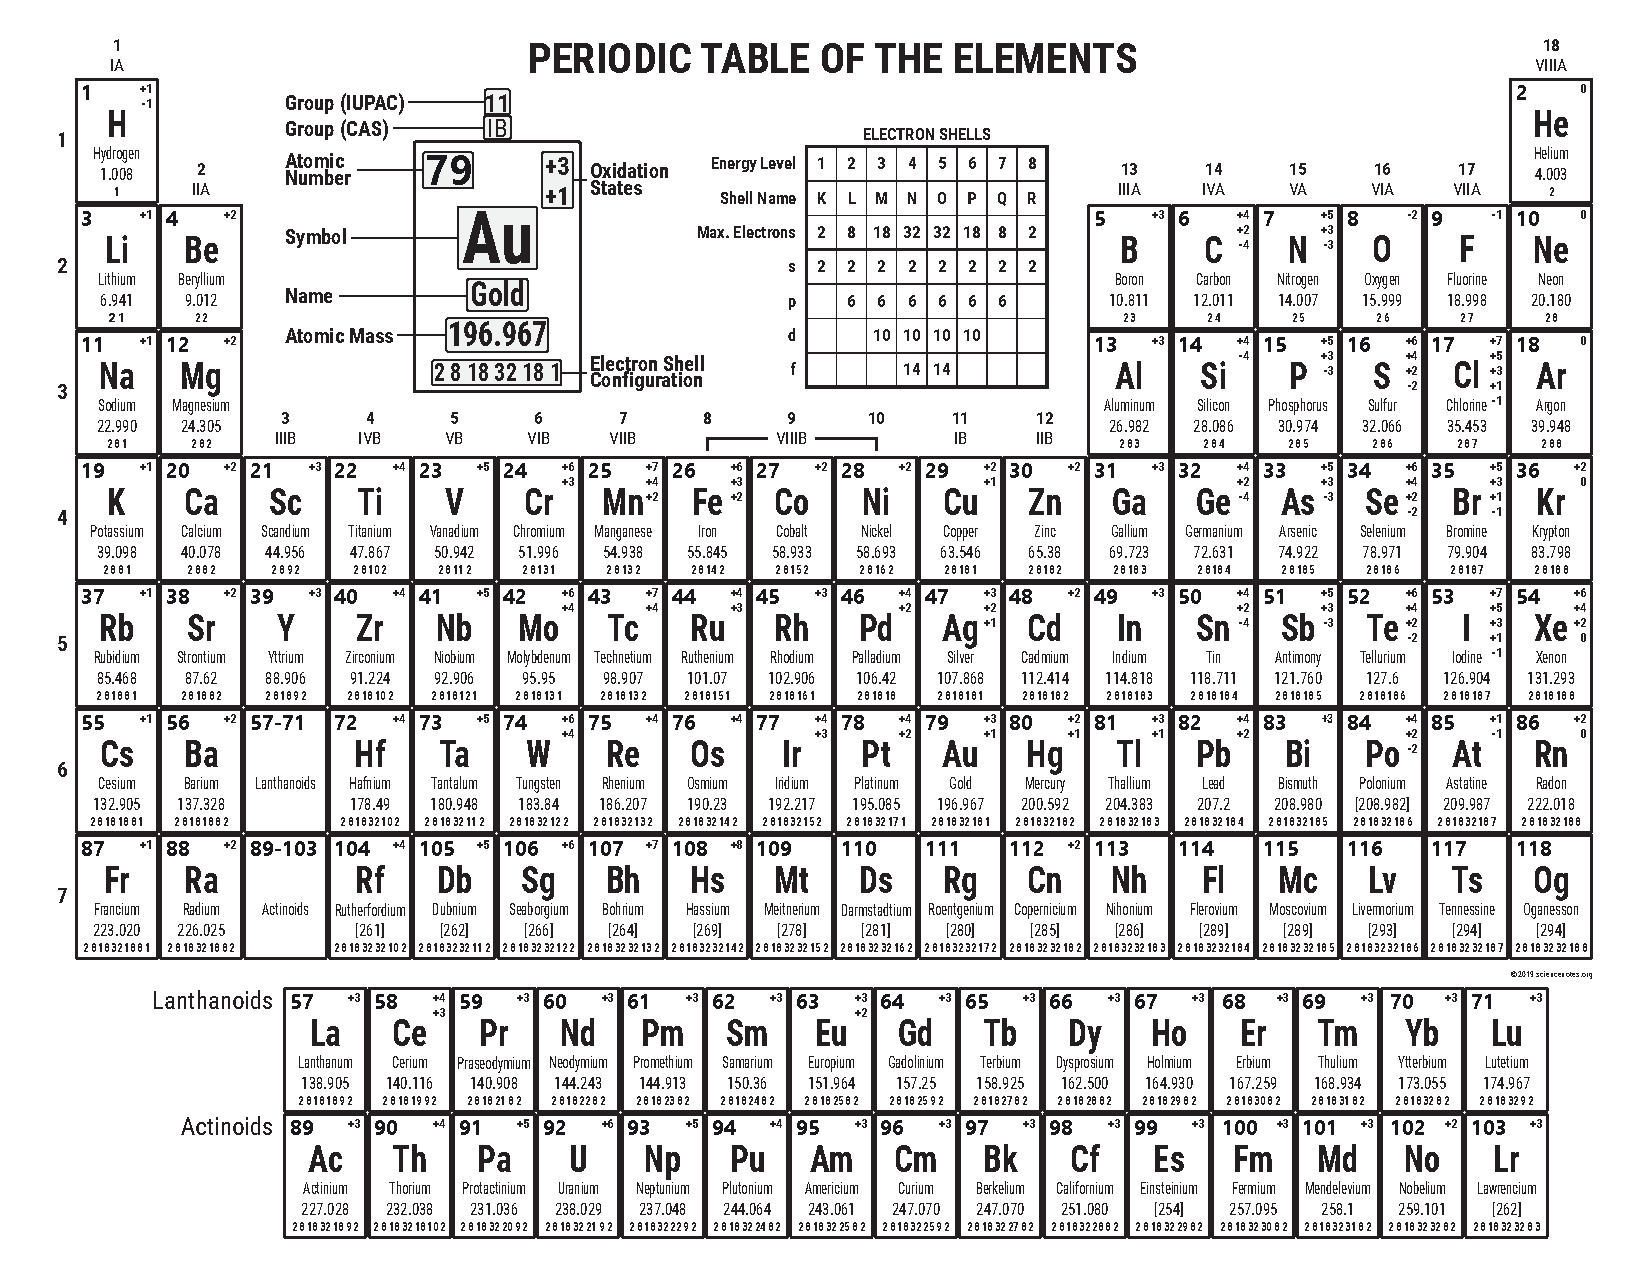
\includepdf[angle=90,pages=-,trim=35mm 10mm 15mm 15mm,width=\textwidth]{assets/PeriodicTableElements.pdf}

\end{document}
